\pdfoutput=1
\documentclass[11pt,a4paper]{article}
\usepackage[hmargin=26mm,vmargin=25mm]{geometry}
\usepackage{amsmath,amssymb,amsthm}
\usepackage{enumitem}
\SetEnumitemKey{titledsteps}{
    label=\arabic*., leftmargin=1.85em, labelsep=.55em,
    topsep=4pt plus 1pt minus 1pt, partopsep=0pt,
    itemsep=3pt plus 1pt minus 1pt, parsep=2pt plus 1pt,
    beginpenalty=10000
}
\usepackage{xcolor}
\usepackage{tikz-cd}
\usetikzlibrary{arrows.meta,calc}
\usepackage[section]{placeins}
\tikzcdset{diagrams={labels={font=\small}}}
\setlength{\abovecaptionskip}{6pt}
\tikzset{
    figwire/.style={-{Latex[length=1.6mm]},line width=.55pt},
    figbox/.style={draw,rounded corners=1.5pt,fill=black!3,
        inner xsep=6pt,inner ysep=4pt,align=center},
    figlabel/.style={font=\footnotesize,inner sep=2pt,fill=white}
}

\usepackage[colorlinks=true,linkcolor=black,citecolor=blue!44!black,urlcolor=blue!44!black]{hyperref}
\setlength{\parskip}{1pt plus .5pt minus .5pt}
\setlength{\textfloatsep}{14pt plus 3pt minus 3pt}
\setlength{\intextsep}{10pt plus 2pt minus 2pt}
\clubpenalty=5000
\widowpenalty=5000
\displaywidowpenalty=5000
\setlength{\emergencystretch}{2em}
\allowdisplaybreaks[1]
\newtheorem{theorem}{Theorem}[section]
\newtheorem{lemma}[theorem]{Lemma}
\newtheorem{proposition}[theorem]{Proposition}
\newtheorem{corollary}[theorem]{Corollary}
\theoremstyle{definition}
\newtheorem{definition}[theorem]{Definition}
\newtheorem*{construction}{Construction}
\newtheorem{example}[theorem]{Example}
\newtheorem{remark}[theorem]{Remark}
\author{%
    Conor Sheridan\\
    \small\href{mailto:siridconor@gmail.com}{\texttt{siridconor@gmail.com}}%
}

\date{\today}

\newcommand{\D}{\mathcal D}
\newcommand{\Pow}{\mathcal P}
\newcommand{\conv}{\operatorname{conv}}
\newcommand{\supp}{\operatorname{supp}}
\newcommand{\one}{\mathbf 1}
\newcommand{\Kl}{\operatorname{Kl}}
\newcommand{\Set}{\mathbf{Set}}
\newcommand{\Opt}{\mathcal O}
\newcommand{\St}{\operatorname{St}}
\newcommand{\Ef}{\operatorname{Ef}}
\title{Independent Randomization and Sequential Composition in Open Games}
\hypersetup{pdftitle={Independent Randomization and Sequential Composition in Open Games},pdfauthor={Conor Sheridan}}

\begin{document}

\maketitle

\begin{abstract}
    Reassociating a sequence of open games should preserve its equilibria. For the probabilistic open games of Ghani, Kupke, Lambert and Nordvall Forsberg, reassociation can change which joint strategy laws are accepted. Taking the convex hull of independent laws admits correlations that require a shared draw. Averaging a return before applying a coplay row that fails to preserve averages can reverse a strict preference even when all strategy draws are independent. We give an associative composition that carries a return law at each possible input and tests the same strategy lottery at every reachable input. Its equilibria are precisely the joint laws obtained from equilibria of an encoding into ordinary open games by taking the independent product across primitive strategy sets. At \textbf{ordinary point contexts}, the fully right-associated bracketing is the unique bracketing of the original rule that contains all of these equilibria for every choice of games. At those contexts every bracketing agrees with the associative rule on pure profiles.
\end{abstract}

\section{Introduction}

Sequential composition lets us analyse an open game in stages. Associativity requires that grouping the stages in different ways preserve the equilibria. With private randomization, this requirement concerns the joint law of the players' strategies. Consider three indifferent players tossing private fair coins. The last two coins agree with probability $1/2$. Sharing one draw preserves their marginal laws but raises that probability to $1$. Can a change of parentheses alone admit the shared-coin law?

For the probabilistic open games of Ghani, Kupke, Lambert and Nordvall Forsberg (GKLF) \cite{gklf}, the answer is yes. At each binary composition their rule takes a product of strategy laws. To test the downstream lottery, it extends the downstream \textbf{equilibrium menu} from a single input to a probability law on inputs. Even at a point input, this extension takes the convex hull of the menu. When the downstream game consists of two players, their product laws can therefore be mixed by a shared draw. Reassociation determines which players lie downstream. This gives a counterexample to the associativity claim in \cite[Theorem~15]{gklf} under the stated reindexing of strategies.

Reassociation can also change the verdict on a fully independent profile. A downstream game returns a fair sign $Z$, and a middle game squares the value it receives. One bracketing averages the sign first and gives $(\mathbb E Z)^2=0$. The other squares it first and gives $\mathbb E[Z^2]=1$. An upstream player who can take a safe payoff of $1/2$ therefore makes opposite strict choices under the two bracketings.

Example~\ref{ex:forget} isolates a difference in the downstream test itself. An \textbf{input-dependent witness} can be forgotten before a later game uses the output, even with singleton backward types.

We interpret private strategy draws by taking the independent product of the players' lotteries. The examples motivate two choices about how to test such a profile. We require each player's lottery over policies to pass its equilibrium test at every reachable input. A sampled policy may still respond to the input it observes. We also retain a probability law for the return at each possible input, so that an upstream coplay can act on that law before the payoff is averaged. Stochastic lenses supply the required states and effects~\cite{bolt}. We use their action on states and effects to encode each probabilistic game as an ordinary open game in Section~\ref{sec:encode}.

The host supplies symmetric monoidal wiring for the encoded primitives. To compare the two serial compositions on the same strategy space, Section~\ref{sec:intrinsic} constructs the associative rule directly on joint laws. Theorem~\ref{thm:direct} identifies its equilibria with the independent products of the lotteries in a host equilibrium profile. A primitive may itself admit a correlated law on a tuple of strategies.

Theorem~\ref{thm:comb} classifies the original bracketings at ordinary point contexts. Only the fully right-associated bracketing contains every equilibrium of the associative rule for every choice of games. All bracketings agree with it on pure profiles. Proposition~\ref{prop:tensor} compares the host tensor with the GKLF parallel rule at ordinary point contexts. Section~\ref{sec:signals} also distinguishes independent strategy draws from actions correlated by a shared observation. Section~\ref{sec:related} compares these results with determinisation, convex closure and stochastic lenses.

\section{Probabilistic games and their serial test}\label{sec:rule}

Two operations on probability laws enter the GKLF serial test. Independent sampling forms a product of two laws, and mixing flattens a law on laws. We use the finitely supported distribution monad $\D$ on $\Set$ for both operations. Write $\delta_x$ for unit mass at $x$, $f_*p$ for pushforward, and $\one$ for a singleton. The double strength $\D A\times\D B\to\D(A\times B)$ sends $(p,q)$ to the independent product $p\otimes q$, with mass $p(a)q(b)$ at $(a,b)$. The monad multiplication flattens a law on laws by $\mu_X(\sum_i t_i\delta_{p_i})=\sum_i t_i p_i$. All sums omit zero-weight terms.

Each backward type $R$ of a probabilistic game carries a $\D$-algebra $\alpha_R:\D R\to R$ satisfying $\alpha_R\delta=\mathrm{id}$ and $\alpha_R\mu=\alpha_R\D\alpha_R$. For real payoffs, $\alpha_R$ is expectation.

A probabilistic open game $G:(X,S)\to(Y,R)$ has a strategy set $A$, a play map $P_G:A\times X\to Y$, a coplay map $C_G:A\times X\times R\to S$, and a context-dependent equilibrium menu
\[
    E_G(x,k)\subseteq\D A,\qquad k:Y\to R.
\]
In the context $(x,k)$, the input $x$ determines where play starts, and the continuation $k$ assigns a return to every possible output. Coplay carries the return at the played output back to the input. The menu $E_G(x,k)$ can be any subset of $\D A$ \cite[Definition~3]{gklf}.

A \textbf{strategic equivalence} is a bijection of strategies that preserves play and coplay and whose pushforward identifies the menus at every context. In particular, the canonical bijection $((a,b),c)\mapsto(a,(b,c))$ must transport the verdict on \emph{every} joint law on triples if serial composition is associative.

\begin{construction}[GKLF serial composition]\leavevmode
    \begin{enumerate}[titledsteps]
        \item \textbf{Compose the pure lenses.} Take $H:(Y,R)\to(Z,T)$ with strategies $B$, and write $G;H$ in order of play. Each $a\in A$ determines a set-based lens $(P_G(a,-),C_G(a,-,-))$. At $(a,b)$, the forward leg of the composite is $P((a,b),x)=P_H(b,P_G(a,x))$. The backward leg is $C((a,b),x,t)=C_G(a,x,C_H(b,P_G(a,x),t))$. At fixed $b$, precomposing the effect $k:Z\to T$ with $H_b$ gives the return at each $y$ (Figure~\ref{fig:serial}).

        \item \textbf{Test the two strategy lotteries.} For candidate lotteries $p\in\D A$ and $q\in\D B$, their joint law is $p\otimes q$, and the input law for $H$ is $\nu=(P_G(-,x))_*p$. Averaging the downstream coplay against $q$ gives the first equilibrium condition of \cite[Definitions~11--12]{gklf},
        \begin{equation}
            p\in E_G(x,k_q),\qquad k_q(y)=\alpha_R\bigl((b\mapsto C_H(b,y,k(P_H(b,y))))_*q\bigr).
            \label{eq:up}
        \end{equation}

        The second condition lifts the downstream menu to the input law $\nu$,
        \begin{equation}
            q\in\D^\#(y\mapsto E_H(y,k))(\nu).
            \label{eq:down}
        \end{equation}
        Every accepted law factors across the two strategy sets at this node. Either strategy set may already consist of tuples.
    \end{enumerate}
\end{construction}

\begin{figure}[!htbp]
    \centering\small
    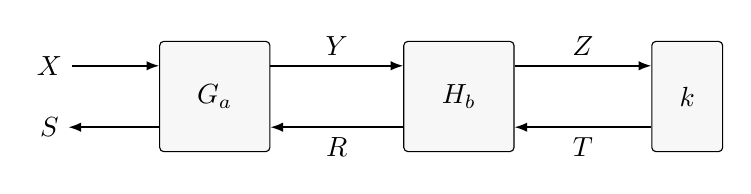
\begin{tikzpicture}[x=1cm,y=1cm]
        \node[figbox,minimum width=14mm,minimum height=14mm] (g) at (0,0) {$G_a$};
        \node[figbox,minimum width=14mm,minimum height=14mm] (h) at (3.1,0) {$H_b$};
        \foreach \v/\yy in {X/.39,S/-.39}
            \node (l\v) at (-2.1,\yy) {$\v$};
        \draw[figwire] (lX) -- ([yshift=3.9mm]g.west);
        \draw[figwire] ([yshift=3.9mm]g.east) -- node[above] {$Y$} ([yshift=3.9mm]h.west);
        \draw[figwire] ([yshift=-3.9mm]h.west) -- node[below] {$R$} ([yshift=-3.9mm]g.east);
        \draw[figwire] ([yshift=-3.9mm]g.west) -- (lS);
        \node[figbox,minimum width=9mm,minimum height=14mm] (k) at (6,0) {$k$};
        \draw[figwire] ([yshift=3.9mm]h.east) -- node[above] {$Z$} ([yshift=3.9mm]k.west);
        \draw[figwire] ([yshift=-3.9mm]k.west) -- node[below] {$T$} ([yshift=-3.9mm]h.east);
    \end{tikzpicture}
    \caption{The forward wires carry play and the backward wires carry coplay. Following the two wires between $H_b$ and the effect $k$ gives $C_H(b,y,k(P_H(b,y)))$ at a proposed $y$.}\label{fig:serial}
\end{figure}

GKLF define the \textbf{downstream lift} \eqref{eq:down} both by a coupling and by finite witnesses \cite[Definition~11]{gklf}. A coupling witnesses that its marginals are related by the Barr lifting of the membership relation along $\D$ \cite[Section~2]{barr}. The induced transformation $\lambda:\D\Pow\Rightarrow\Pow\D$ is natural by Kupke, Kurz and Venema \cite[Fact~3.14]{kkv}, as GKLF note in Fact~14. Goy and Petri\c{s}an identify this transformation as a weak distributive law \cite[Theorem~3.2]{goy}. GKLF already observe that $\lambda$ fails the distribution-unit law. We compute the effect of that failure on the menu of a game.

\begin{construction}[The downstream lift]\leavevmode
    \begin{enumerate}[titledsteps]
        \item \textbf{Choose a coupling.} For $T:X\to\Pow(\D A)$ and $\eta\in\D X$, the law $T_*\eta$ records the menus seen at the input. Given a law $\xi$ on subsets of $V$, let $\lambda_V(\xi)$ be the set of second marginals of all finitely supported couplings on $\Pow V\times V$ with first marginal $\xi$ and support in $\{(U,v):v\in U\}$. Apply this construction at $V=\D A$ and $\xi=T_*\eta$.

        \item \textbf{Flatten its second marginal.} For each $\gamma\in\lambda_{\D A}(T_*\eta)$, apply the monad multiplication. This yields
        \begin{equation}
            \D^\#T(\eta)=\{\,\mu_A(\gamma):\gamma\in
            \lambda_{\D A}(T_*\eta)\,\}.
            \label{eq:lambda}
        \end{equation}
        The intermediate law $\gamma$ is a distribution on \textbf{lotteries}. Choosing an element of a menu and flattening are distinct steps of the definition.
    \end{enumerate}
\end{construction}

Figure~\ref{fig:membership} locates the choice in this construction. The input law fixes the first marginal of a witness on the membership relation. Projecting to the second marginal and flattening gives one admissible lottery for each such witness.

\begin{figure}[!htbp]
    \centering\small
    \begin{tikzcd}[column sep=large,row sep=large]
        \D X \arrow[r,"T_*"] &
        \D\Pow(\D A) &
        \D M_A \arrow[l,"(\pi_1)_*"'] \arrow[r,"(\pi_2)_*"] &
        \D^2 A \arrow[r,"\mu_A"] & \D A
    \end{tikzcd}
    \caption{The membership span for $M_A=\{(U,\rho)\mid U\subseteq\D A,\ \rho\in U\}$. Fix the value $T_*\eta$ at the second node. Every law on $M_A$ in its fibre gives one output by the two rightward arrows.}\label{fig:membership}
\end{figure}

\section{Convex closure and the input identity}\label{sec:unit}

Inserting an identity before a game supplies a point input to its downstream test. Goy and Petri\c{s}an give the row decomposition of the membership lifting \cite[Lemma~3.1]{goy}. Applying it to a distribution on menus and flattening each row gives the following formula for the GKLF lift. Write $\conv M$ for finite convex closure, with $\conv\varnothing=\varnothing$. A weighted sum of sets consists of the sums obtained by choosing one element from each positive-weight set.

\begin{lemma}[Finite witnesses]\label{lem:lift}
    For $\eta\in\D X$ and $T:X\to\Pow(\D A)$,
    \begin{equation}
        \D^\# T(\eta)=
        \sum_{x\in\supp\eta}\eta(x)\conv T(x).
        \label{eq:weighted}
    \end{equation}
    In particular $\D^\# T(\delta_x)=\conv T(x)$.
\end{lemma}
\begin{proof}\leavevmode
    \begin{enumerate}[titledsteps]
        \item \textbf{From input rows to a coupling.} A finite family $(w_{xj},\rho_{xj})$ with $w_{xj}>0$, $\rho_{xj}\in T(x)$ and row sums $\sum_jw_{xj}=\eta(x)$ gives a coupling in \eqref{eq:lambda} by placing mass $w_{xj}$ at $(T(x),\rho_{xj})$, adding coincident entries. Flattening the second marginal of this coupling gives $\sum_{xj}w_{xj}\rho_{xj}$.

        \item \textbf{From a coupling to input rows.} Conversely let $\omega$ be a witnessing coupling. For each $x\in\supp\eta$ and each $\rho$ with $\omega(T(x),\rho)>0$, put
        \[
            w_{x,\rho}=\eta(x)\frac{\omega(T(x),\rho)}{(T_*\eta)(T(x))}.
        \]
        The denominator is positive. Summing over $\rho$ recovers $\eta(x)$, while summing over the $x$ sharing one value of $T(x)$ recovers the original coupling row. Thus flattening is unchanged.

        Each positive row, after division by its mass, gives an element of $\conv T(x)$. Conversely, expanding a chosen element of each convex hull and multiplying its coefficients by $\eta(x)$ recovers a row witness. This proves \eqref{eq:weighted}. A positively weighted empty menu makes both sides empty. For $\eta=\delta_x$ the only positive row has weight one, so the lift is $\conv T(x)$.\qedhere
    \end{enumerate}
\end{proof}

At a point input the coupling still has a choice of lotteries within a single menu. Figure~\ref{fig:unit} identifies the resulting operation as convex closure. This determines exactly when precomposition by an identity preserves the menu.

\begin{figure}[!htbp]
    \centering\small
    \begin{tikzcd}[column sep=19mm,row sep=9mm]
        X \arrow[r,"T"] \arrow[d,"\delta_X"'] &
        \Pow(\D A) \arrow[d,"\conv"]\\
        \D X \arrow[r,"\D^\#T"'] & \Pow(\D A)
    \end{tikzcd}
    \caption{Point inputs and convex closure. The square commutes for every menu-valued map $T$. Replacing its right edge by the identity preserves commutativity exactly when every $T(x)$ is convex.}\label{fig:unit}
\end{figure}

\begin{proposition}[Input identity]\label{prop:unit}
    Precomposing $H$ by the identity changes its menu at $(y,k)$ to $\conv E_H(y,k)$ under $\one\times B\cong B$. It preserves every verdict of $H$ precisely when every such menu is convex.
\end{proposition}
\begin{proof}
    The identity plays its input, copies the return, and accepts its unique strategy. Its output law at $y$ is therefore $\delta_y$. The upstream test \eqref{eq:up} holds automatically, while Lemma~\ref{lem:lift} turns \eqref{eq:down} into membership in $\conv E_H(y,k)$. This agrees with the original menu precisely when that menu is convex. In the opposite order the unique downstream lottery is always admitted, and the expected identity coplay is $k$ since $\alpha_T\delta=\mathrm{id}$.
\end{proof}

The extended proof of GKLF's Lemma~16 simplifies the lift of a constant singleton menu when computing the input identity \cite[p.~15]{extended}. That calculation applies when the identity is downstream. In $\mathrm{id};H$, the downstream menu is $E_H(-,k)$ and its lift at $\delta_y$ is $\conv E_H(y,k)$.

\begin{construction}[Identity insertion for binary games]
    For a binary strategy set with menu $\{\delta_0,\delta_1\}$, inserting the input identity adds the fair lottery. The same change can occur after composing games whose primitive menus are convex.

    Take two indifferent binary games with singleton external interfaces. Their menus are both $\D\{0,1\}$. The tensor equilibrium rule \cite[Definition~5]{gklf} accepts every product of the two lotteries, since both marginal tests are automatic. In particular the tensor accepts $\delta_{(0,0)}$ and $\delta_{(1,1)}$, so its convex hull contains their fair mixture. It assigns zero mass to $(0,1)$, whereas the product of its fair marginals assigns $1/4$. Inserting the input identity thus changes the verdict on this joint law.
\end{construction}

This example also tests the interchange equation asserted in \cite[Lemma~17]{gklf}. Write $U,V$ for the two indifferent games and $e$ for the identity on the singleton interface. Compare
\[
    (e;U)\otimes(e;V)
    \qquad\text{and}\qquad
    (e\otimes e);(U\otimes V).
\]
On the left, the two primitive menus are convex, so Proposition~\ref{prop:unit} leaves them unchanged and the tensor admits exactly the product laws. On the right, $e\otimes e$ is the identity under the singleton reindexings. The downstream lift convexifies the product menu. That menu contains every joint point mass, so its convex hull is the entire simplex. The fair diagonal law distinguishes the two sides.

\paragraph{Naturality after flattening.}

The row formula also determines which maps can be applied before or after the downstream lift. For $f:\D A\to\D B$, write $f[M]$ for the direct image of a menu. The identity
\[
    f\bigl[\D^\#T(\eta)\bigr]
    =\D^\#\bigl(x\mapsto f[T(x)]\bigr)(\eta)
\]
holds for all $X,T,\eta$ exactly when $f$ is a morphism of free $\D$-algebras.

\begin{proof}
    If $f$ is affine, applying it to a witness in \eqref{eq:weighted} applies $f$ to each lottery in the witness and leaves the weights unchanged. Conversely any witness formed from the image menus uses finitely many images, for which we may take preimages in the corresponding menus. This proves the identity. If the identity holds for all menus, take $T(i)=\{p_i\}$ and $\eta(i)=t_i$. Then $f(\sum_i t_ip_i)=\sum_i t_if(p_i)$ for every finite convex combination, so $f$ is affine. In particular, the marginal maps used after Fact~14 of \cite{gklf} do satisfy this identity.
\end{proof}

\section{A failure of sequential associativity}\label{sec:assoc}

Convex closure affects associativity because a product of two menus can have a nonconvex image among joint laws. To isolate that effect, take games on $(\one,\one)\to(\one,\one)$. They have a single context and their play and coplay are unique.

Write $U_A$ for the \textbf{indifferent game} with strategy set $A$ and menu $\D A$. More generally, if two games on this interface have menus $M\subseteq\D A$ and $N\subseteq\D B$, equations~\eqref{eq:up}--\eqref{eq:down} and Lemma~\ref{lem:lift} give
\begin{equation}
    M\star N=\{p\otimes q:p\in M,\ q\in\conv N\}.
    \label{eq:star}
\end{equation}

\begin{theorem}[Equilibria under the two bracketings]\label{thm:assoc}
    For nonempty finite sets $A,B,C$, identify both bracketings of the strategy set with $A\times B\times C$. The accepted laws are exactly
    \begin{align*}
        (U_A;U_B);U_C &: \quad
        \{p\otimes q\otimes r:p\in\D A,\ q\in\D B,\ r\in\D C\},\\
        U_A;(U_B;U_C) &: \quad
        \{p\otimes s:p\in\D A,\ s\in\D(B\times C)\}.
    \end{align*}
    The inclusion from the first set into the second is strict when $|B|,|C|\ge2$.
\end{theorem}
\begin{proof}
    At two indifferent leaves the right menu is already convex. Hence \eqref{eq:star} accepts exactly the products of their strategy laws. At the root of the left bracketing, the $AB$ menu is the left argument of $\star$. Equation~\eqref{eq:star} preserves that product constraint and takes an independent product with the law on $C$. In the right bracketing the $BC$ menu is the right argument of $\star$. Its convex hull is all of $\D(B\times C)$ because it contains every point mass $\delta_{(b,c)}=\delta_b\otimes\delta_c$.

    To see strictness choose two distinct labels $0,1$ in each of $B,C$. The law $d=(\delta_{(0,0)}+\delta_{(1,1)})/2$ has fair marginals and $d(0,1)=0$. The product of its marginals has mass $1/4$ there. For any $p$, the $BC$-marginal of $p\otimes d$ is $d$, so it cannot factor into the three required laws.
\end{proof}

Figure~\ref{fig:brackets} shows how the position of a product menu determines whether its independence constraint survives the next composition.

\begin{figure}[!htbp]
    \centering\small
    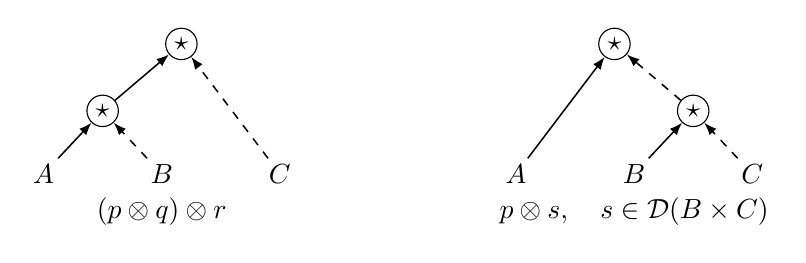
\begin{tikzpicture}[x=1cm,y=1cm,
        branch/.style={figwire}, closure/.style={figwire,dashed},
        op/.style={circle,draw,fill=white,inner sep=1.6pt},leaf/.style={inner sep=2pt}]
        \begin{scope}
            \node[leaf] (a) at (0,0) {$A$}; \node[leaf] (b) at (1.5,0) {$B$};
            \node[leaf] (c) at (3,0) {$C$};
            \node[op] (ab) at (.75,.8) {$\star$}; \node[op] (abc) at (1.75,1.65) {$\star$};
            \draw[branch] (a)--(ab); \draw[closure] (b)--(ab);
            \draw[branch] (ab)--(abc); \draw[closure] (c)--(abc);
            \node at (1.5,-.48) {$(p\otimes q)\otimes r$};
        \end{scope}
        \begin{scope}[xshift=6cm]
            \node[leaf] (a) at (0,0) {$A$}; \node[leaf] (b) at (1.5,0) {$B$};
            \node[leaf] (c) at (3,0) {$C$};
            \node[op] (bc) at (2.25,.8) {$\star$}; \node[op] (abc) at (1.25,1.65) {$\star$};
            \draw[branch] (b)--(bc); \draw[closure] (c)--(bc);
            \draw[branch] (a)--(abc); \draw[closure] (bc)--(abc);
            \node at (1.5,-.48) {$p\otimes s,\quad s\in\D(B\times C)$};
        \end{scope}
    \end{tikzpicture}
    \caption{Read each tree upwards. A dashed edge convexifies its child's menu before the product is formed at $\star$. Only in the right-hand tree does the $BC$ product menu itself travel along a dashed edge.}\label{fig:brackets}
\end{figure}

GKLF distinguish product strategies from general joint laws after Definition~5 and ask in their conclusion whether non-independent laws can model correlated equilibrium \cite[pp.~98 and~104]{gklf}. For three binary players, let $u$ be the first player's fair law and let $d$ be the diagonal law in the proof. The right bracketing accepts $u\otimes d$ and the left rejects it.

The extended proof of GKLF's Theorem~15 compares $(p\otimes q)\otimes r$ with $p\otimes(q\otimes r)$ \cite[Appendix, pp.~14--15]{extended}. A comparison restricted to triple products omits precisely the kind of law that distinguishes these menus.

Could a different bijection of the eight pure profiles identify these two menus? Counting the two-point supports in each menu rules out every such bijection.

\begin{proof}
    A product law has support equal to the product of its marginal supports. Hence a two-point support in the fully independent menu is an edge of the binary cube. There are $3\cdot 4=12$ such edges.

    In the second menu a two-point support either fixes $a$ or fixes $(b,c)$, since the law factors across these two coordinates. At fixed $a$, choosing two of the four pairs $(b,c)$ gives $2\binom{4}{2}=12$ supports. Varying $a$ at fixed $(b,c)$ gives another four. Fair mixtures realize all these supports. A bijection of pure profiles preserves support cardinality, so it cannot identify menus with $12$ and $16$ two-point supports, respectively.
\end{proof}

Fix an external context and write $A_T$ for the pure strategy set of a bracketed expression $T$. An interpretation reads each law as a target profile by a map $j_T:\D A_T\to Q_T$. Write $E_T\subseteq\D A_T$ for the source menu. A target equilibrium predicate $V_T:Q_T\to\{0,1\}$ recovers that menu precisely when $E_T=(V_T\circ j_T)^{-1}(\{1\})$. For the canonical strategy reindexing $\rho:A_T\to A_{T'}$, an associative interpretation \textbf{respects reindexing} when its associator acts on profiles by a bijection $\gamma:Q_T\to Q_{T'}$ satisfying
\[
    \gamma\circ j_T=j_{T'}\circ\rho_*,
    \qquad V_{T'}\circ\gamma=V_T.
\]

\begin{corollary}\label{cor:obstruction}
    An associative interpretation respecting the canonical strategy reindexings cannot recover every joint-law verdict of GKLF serial composition.
\end{corollary}
\begin{proof}
    Let $T=(U_A;U_B);U_C$ and $T'=U_A;(U_B;U_C)$ for three binary strategy sets. Regard $w=u\otimes d$ as a law on $A_T$ under the tuple identification of Theorem~\ref{thm:assoc}. Compatibility with reassociation gives
    \[
        V_T(j_T(w))=V_{T'}(j_{T'}(\rho_*w)).
    \]
    Exact recovery makes the left side false and the right side true by Theorem~\ref{thm:assoc}.
\end{proof}

Proposition~\ref{prop:unit} and Theorem~\ref{thm:assoc} give counterexamples to the identity and associativity claims for the proposed category \cite[Lemma~16 and Theorems~15 and~18]{gklf}. With singleton interfaces, the equilibrium menu accounts for the entire discrepancy. For longer sequences of indifferent players we can identify exactly which groups of strategies remain independent.

\begin{proposition}[Equilibrium laws for a binary tree]
    Let $T$ be a binary bracketing of indifferent singleton-interface games with strategy sets $A_i$. Write $\ell(T)$ for its set of leaves and $\mathbin{\Vert}$ for list concatenation. The ordered list of blocks $\mathcal B(T)$ is given by
    \[
        \mathcal B(i)=[\{i\}],\qquad
        \mathcal B((L,R))=\mathcal B(L)\mathbin{\Vert}[\ell(R)].
    \]
    For $A_B=\prod_{i\in B}A_i$ in leaf order, the equilibrium menu is
    \[
        E_T=\left\{\bigotimes_{B\in\mathcal B(T)}q_B
        \;\middle|\; q_B\in\D A_B\text{ for each }B\in\mathcal B(T)\right\}.
    \]
\end{proposition}
\begin{proof}
    At a leaf $E_i=\D A_i$. By induction using \eqref{eq:star}, every subtree admits every joint point mass, so $\conv E_R=\D A_{\ell(R)}$. At an internal node \eqref{eq:star} therefore gives
    \[
        E_{(L,R)}=\{p\otimes q\mid p\in E_L,\ q\in\D A_{\ell(R)}\}.
    \]
    Substituting the block formula for $E_L$ appends $\ell(R)$ as one block, as required.
\end{proof}

For example, $\mathcal B(((1,2),(3,4)))=[\{1\},\{2\},\{3,4\}]$. The joint law has the form $q_1\otimes q_2\otimes q_{34}$, with arbitrary dependence between the last two strategies.

\section{A preference reversal on independent profiles}\label{sec:reversal}

The preceding example separates the two bracketings by a correlated strategy law. We now fix independent strategy draws throughout and compare the continuation received by the first player. GKLF's extended proof identifies the two continuations after expanding composite play and coplay \cite[p.~14, proof of Theorem~15]{extended}. A nonlinear coplay makes their order of evaluation observable in a strict choice.

\begin{construction}[Three games for the strict preference reversal]\leavevmode
    \begin{enumerate}[titledsteps]
        \item \textbf{The upstream decision.} Write $s$ for the safe action and $r$ for the risky action. Let $Y=\{s,r\}$ and let $u$ be the fair law on $Z=\{-1,1\}$. Use the usual expectation algebra on $\mathbb R$. $G:(\one,\one)\to(Y,\mathbb R)$ is a decision. Its pure strategy is $y\in Y$, it plays $y$, its coplay is unique, and its menu against $v$ is the set of lotteries maximizing $\sum_y p(y)v(y)$.

        \item \textbf{The middle coplay.} $H:(Y,\mathbb R)\to(Y,\mathbb R)$ has one strategy, transmits $y$ unchanged, and always accepts. Its coplay at $y$ is $h_y(t)$, where $h_s(t)=1/2$ and $h_r(t)=t^2$.

        \item \textbf{The terminal lottery.} The terminal game $I:(Y,\mathbb R)\to(\one,\one)$ has strategies $z\in Z$, unique play, and coplay $C_I(z,y,*)=z$. Its menu is $\{u\}$ at every input, so both bracketings use the same fair sign law. These data satisfy \cite[Definition~3]{gklf}, which gives coplay the type of an ordinary function. All three games have convex equilibrium menus in every context.
    \end{enumerate}
\end{construction}

\begin{theorem}[Strict reversal]\label{thm:reverse}
    At the unique external context the entire menu of $(G;H);I$ is the singleton containing $\delta_s\otimes\delta_*\otimes u$. The menu of $G;(H;I)$ is the singleton containing $\delta_r\otimes\delta_*\otimes u$ under the canonical identification.
\end{theorem}
\begin{proof}\leavevmode
    \begin{enumerate}[titledsteps]
        \item \textbf{Left association.} At the root of $(G;H);I$, equation~\eqref{eq:down} forces the terminal lottery to be $u$, since every reachable row is $\{u\}$. Equation~\eqref{eq:up} gives $G;H$ the constant continuation $y\mapsto\sum_z u(z)z=0$. The inner serial rule then presents $G$ with $y\mapsto h_y(0)$. Its two values are $1/2$ and $0$. The unique best reply is $\delta_s$ and the unique strategy of $H$ passes its test.

        \item \textbf{Right association.} In $G;(H;I)$ the menu of $H;I$ at each $y$ is the singleton $\{\delta_*\otimes u\}$. Its outer lift remains that singleton for every upstream lottery by Lemma~\ref{lem:lift}. Pure composite coplay at $(y,z)$ equals $h_y(z)$. Equation~\eqref{eq:up} therefore presents $G$ with $y\mapsto\sum_z u(z)h_y(z)$. The two values are $1/2$ and $1$, so $\delta_r$ is the unique best reply. The downstream tests all pass. This exhausts the candidate profiles on either side.\qedhere
    \end{enumerate}
\end{proof}

\begin{construction}[Finite backward interfaces]
    The reversal also has a realization with finite interface carriers. Use $V=\{-1,0,1/2,1\}$ at both nontrivial backward ports. Give $V$ the join with top element $0$ and the other three elements pairwise incomparable. Map each law to the join of its support. This is a $\D$-algebra because a Dirac law has singleton support and the support of a mixture is the union of its positive-weight supports.

    Take $h_s$ constant at $1/2$, set $h_r(-1)=h_r(1)=1$ and $h_r(0)=h_r(1/2)=0$. Let $G$ rank lotteries by the usual real expected utility of these numerical labels. The fair sign has join $0$ and its image under $h_r$ is $\delta_1$. Consequently the left and right risky values are again $0$ and $1$, with $1/2$ on safe. All pure strategy sets and interface carriers in this realization are finite.
\end{construction}

Squaring a fair sign gives different results depending on when the return is averaged. The following criterion identifies all backward maps for which the two orders of evaluation agree.

\begin{proposition}[Interchange with a backward map]\label{prop:affine}
    For a fixed row $h:T\to R$ between backward types, averaging before and after that row gives the same value for every finitely supported downstream law precisely when $h$ is a $\D$-algebra morphism. Each failure of this identity is realizable by a terminal random-return game and a deterministic middle game.
\end{proposition}
\begin{proof}
    Given $\rho\in\D T$, the two maps give $h(\alpha_T(\rho))$ and $\alpha_R(h_*\rho)$. Equality on all $\rho$ is exactly $h\alpha_T=\alpha_R\D h$.

    To realize the two evaluations, take singleton forward interfaces and a middle game with one strategy and coplay $h$. Give the final game strategy set $\supp\rho$, menu $\{\rho\}$ on that support, and coplay equal to its strategy value. Equations~\eqref{eq:up}--\eqref{eq:down} then yield $h(\alpha_T(\rho))$ and $\alpha_R(h_*\rho)$ in the respective bracketings. If these values differ, a binary upstream game separates them by admitting $\delta_0$ exactly when its continuation at the unique output equals the first value. The real-valued decision of Theorem~\ref{thm:reverse} realizes this distinction as a strict preference.
\end{proof}

Figure~\ref{fig:affine} evaluates the interchange from Proposition~\ref{prop:affine} on the return law in Theorem~\ref{thm:reverse}.

\begin{figure}[!htbp]
    \centering\small
    \begin{tikzcd}[column sep=large,row sep=large]
        \D T \arrow[r,"\D h"] \arrow[d,"\alpha_T"'] & \D R \arrow[d,"\alpha_R"]\\
        T \arrow[r,"h"'] & R
    \end{tikzcd}\hspace{10mm}%
    \begin{tikzcd}[column sep=8mm,row sep=6mm]
        & \delta_1 \arrow[r,"\mathbb E"] & 1\\
        \rho \arrow[ur,"(h_r)_*"] \arrow[dr,"\mathbb E"'] &&\\
        & 0 \arrow[r,"h_r"'] & 0
    \end{tikzcd}
    \caption{An algebra morphism makes the square on the left commute. On the right, the two paths starting at the fair-sign law $\rho$ end at $1$ and $0$ for $h_r(t)=t^2$.}\label{fig:affine}
\end{figure}

\begin{proof}[Derivation of the rowwise interchange]
    Let $q$ be a fixed middle strategy law and let $\rho_z$ be the downstream return law at forward value $z$ under a fixed final strategy law and continuation. At a proposed upstream $y$, put $z_b=P_H(b,y)$ and $h_b=C_H(b,y,-)$. Expanding \eqref{eq:up} on the two sides gives respectively
    \[
        \alpha_R\!\left(\sum_b q(b)\delta_{h_b(\alpha_T\rho_{z_b})}\right),
        \qquad
        \alpha_R\!\left(\sum_b q(b)(h_b)_*\rho_{z_b}\right).
    \]

    If each row preserves finite averages, substitute $\alpha_R((h_b)_*\rho_{z_b})$ for $h_b(\alpha_T\rho_{z_b})$ in the first expression. The algebra identity $\alpha_R\D\alpha_R=\alpha_R\mu_R$ then gives the second. At the given $y$, the two orders therefore agree for every middle lottery $q$ and every family of downstream return laws exactly when each row $C_H(b,y,-)$ is a $\D$-algebra morphism. For necessity, take $q=\delta_b$ and the constant downstream family $z\mapsto\rho$. Varying $\rho$ recovers the row identity of Proposition~\ref{prop:affine}.

    The quantifier over $q$ matters. For a fixed fair lottery on two strategies with the same play output, take real returns and coplays $h_+(t)=t^2$ and $h_-(t)=-t^2$. For any downstream law $\rho$, the two contributions cancel in each displayed expression. Both expressions are zero, although each row fails the algebra identity on a fair sign.
\end{proof}

GKLF discuss compatibility of coutility with the distribution algebra when considering functoriality of determinisation \cite[discussion following Proposition~20]{gklf}. Proposition~\ref{prop:affine} locates the same algebra equation inside the upstream serial test. The downstream test can also distinguish independent profiles, even when all backward types are singletons.

\begin{example}[Forgetting an input-dependent witness]\label{ex:forget}
    Let $U=\{0,1\}$, write $u$ for the fair law on $U$, and write $\oplus$ for addition modulo two. All backward types are $\one$. The first game $G$ has singleton input, plays its bit $a$, and admits only $u$. At input $y\in U$ the second game $H$ has strategy bit $b$, plays $y\oplus b$, and has menu $\{\delta_y\}$. At input $z\in U$ the third game $I$ has strategy bit $c$, singleton output, and menu $\{\delta_z\}$. Every primitive menu is a convex singleton.

    In $(G;H);I$, the lift for $H$ averages $\delta_y$ over the fair input, so $G;H$ records $u\otimes u$ on $(a,b)$. The bits in that product are independent, hence $z=a\oplus b$ is fair. The lift for $I$ then forces $c\sim u$. In $G;(H;I)$, fix $y$ before composing the suffix. The test for $H$ forces $b=y$, so $z=0$ and $c=0$. The suffix menu is $\{\delta_{(y,0)}\}$. Its lift over $y\sim u$ gives the single law $u\otimes\delta_0$ on $(b,c)$. Thus the entire menus, in strategy order $(a,b,c)$, are
    \[
        \{u\otimes u\otimes u\}
        \qquad\text{and}\qquad
        \{u\otimes u\otimes\delta_0\},
    \]
    respectively. Both contain only independent profiles. The difference is whether the equality $b=y$ in the lift witness survives until the output $y\oplus b$ is evaluated.
\end{example}

\section{An encoding into ordinary open games}\label{sec:encode}

For the upstream test, we keep the return law until the primitive game asks for a payoff. For the downstream test, we keep the strategy lottery fixed as the input varies over its support. The first choice determines the interface of the encoding. The second determines its equilibrium menu.

Let $\mathcal K=\Kl(\D)$, and let $\Opt$ be its category of coend lenses, with tensor unit $I=(\one,\one)$. An interface $U=(X,S)$ has states $\St(U)=\Opt(I,U)$ and effects $\Ef(U)=\Opt(U,I)$. Their standard descriptions are
\begin{equation}
    \St(X,S)\cong\mathcal K(\one,X)\cong\D X,\qquad
    \Ef(X,S)\cong\mathcal K(X,S)=\Set(X,\D S).
    \label{eq:state-effect}
\end{equation}
Terminality of $\one$ in $\mathcal K$ gives the state isomorphism. For effects, co-Yoneda composes the two legs of a representative. These are Riley's state and costate formulas \cite[Propositions~2.0.6--2.0.7]{riley}, specialized to stochastic lenses as in Bolt, Hedges and Zahn \cite[Lemmas~3.5.1 and~3.12.1]{bolt}. An effect is thus a table assigning a return law to every possible input, including inputs outside the support of the state.

Fixing a strategy lottery gives a stochastic lens. Its action on states propagates the input law, and its action on effects pulls back a \textbf{return table}. Appendix~\ref{app:optic} derives both actions from the coend. Definition~\ref{def:encode} uses them as the play and coplay of an ordinary open game.

In the ordinary open games that serve as our host \cite{pure}, an equilibrium function selects elements of the strategy set \cite[Definition~1 and Theorem~2]{gklf}. The following observation lets us use that presentation also when the host is defined by best-response relations.

\begin{construction}[The \textbf{diagonal best-response relation}]
    For each context, associate to its menu the relation $\{(a,a)\mid a\text{ is accepted}\}$. Both serial and parallel composition test the two component relations simultaneously. The relation on a pair of strategies is therefore diagonal, and a pair lies on that diagonal exactly when both component tests pass. Thus the relational presentation realizes the equilibrium functions used below.
\end{construction}

\begin{definition}[Encoding a primitive]\label{def:encode}
    For an interface $(X,S)$, let
    \[
        F(X,S)=(\D X,\,X\to\D S).
    \]
    The two components are the state and effect sets in \eqref{eq:state-effect}. For a game $G:(X,S)\to(Y,R)$ with strategy set $A$, its \textbf{encoding} is the ordinary open game $G^\sharp:F(X,S)\to F(Y,R)$ with strategy set $\D A$. At $p\in\D A$ and $\eta\in\D X$, its play is
    \begin{equation}
        P^\sharp_G(p,\eta)=\sum_{x,a}\eta(x)p(a)\delta_{P_G(a,x)}.
        \label{eq:play}
    \end{equation}
    For a return table $r:Y\to\D R$, its coplay assigns to each $x\in X$ the law
    \begin{equation}
        C^\sharp_G(p,\eta,r)(x)=\sum_{a,t}p(a)r(P_G(a,x))(t)\delta_{C_G(a,x,t)}.
        \label{eq:coplay}
    \end{equation}
    A \textbf{host continuation} $\kappa:\D Y\to(Y\to\D R)$ selects a return table at the point state $\delta_y$. Evaluating its row at $y$ gives the ordinary continuation $k^\flat_\kappa:Y\to R$,
    \begin{equation}
        k^\flat_\kappa(y)=\alpha_R(\kappa(\delta_y)(y)).
        \label{eq:flat}
    \end{equation}
    The equilibrium menu tests the same lottery at each supported input. Bolt, Hedges and Zahn use a supportwise optimality test for Bayesian policies \cite[Definition~4.4.1]{bolt}. Here the test applies to an arbitrary primitive menu,
    \begin{equation}
        E_{G^\sharp}(\eta,\kappa)=\bigcap_{x\in\supp\eta}E_G(x,k^\flat_\kappa).
        \label{eq:common}
    \end{equation}
\end{definition}
\begin{proof}[Well-definedness of the encoding]
    The forward law in \eqref{eq:play} and each coplay row in \eqref{eq:coplay} have total mass one. For a fixed coplay input $x_0$, the two normalizations are
    \[
        \begin{aligned}
            \sum_{x,a}\eta(x)p(a)
            &= \Bigl(\sum_x\eta(x)\Bigr)\Bigl(\sum_a p(a)\Bigr)=1,\\
            \sum_a p(a)\sum_t r(P_G(a,x_0))(t)
            &= \sum_a p(a)=1 .
        \end{aligned}
    \]
    The forward sum has finite support because $\eta$ and $p$ do. In each coplay row, $p$ selects only finitely many strategies, each of which reads a finitely supported return law.

    In the coplay formula a single draw of $a$ chooses both the return row at $P_G(a,x)$ and the map $C_G(a,x,-)$ applied to that return. This defines a return law for every $x$, including those with $\eta(x)=0$, since the factor $\eta(x)$ occurs only in the forward sum.
\end{proof}

For a decision whose pure strategies are policies $f:X\to Y$ and whose play is $P(f,x)=f(x)$, a lottery $p\in\D(Y^X)$ induces the behavioural policy
\[
    \sigma_p(x)=(\mathrm{ev}_x)_*p,\qquad
    \mathrm{ev}_x(f)=f(x).
\]
Take a common real-valued payoff $v:Y\to\mathbb R$ and let $E_G(x,v)$ admit $p$ when $\sigma_p(x)$ maximizes the expectation of $v$ over $\D Y$. Then \eqref{eq:common}, at $k^\flat_\kappa=v$, gives the positive-support test of Bolt, Hedges and Zahn \cite[Definition~4.4.1]{bolt} for a singleton latent state. Hedges's earlier stochastic decision \cite[Section~2.1.8]{hedges} gives the same test in its finite-action setting. Write $v(y)$ for the expected return from action $y$ and $m=\max_y v(y)$. For a behavioural policy $\sigma$, its expected payoff is
\[
    \sum_{x\in\supp\eta}\eta(x)\sum_y\sigma(x)(y)v(y)\ \leq\ m .
\]
Hedges's criterion requires this value to be at least $m$. Each inner sum is at most $m$, so the criterion holds exactly when every positive-weight row attains $m$.

The relation between behavioural strategies and lotteries on complete contingent plans goes back to Kuhn \cite{kuhn} and is discussed for Bayesian open games in \cite[Section~4.6, footnote~5]{bolt}. At a given observation $x$, only the evaluation marginal $(\mathrm{ev}_x)_*p$ enters this decision's payoff. Every family of behavioural rows $\sigma(x)$ on the finite set $S=\supp\eta$ is realized there by a lottery on policies. Draw a table under $\bigotimes_{x\in S}\sigma(x)$ and extend it to $X$ by copying its value at one fixed $x_0\in S$ to every input outside $S$. The evaluation marginals on $S$ are the prescribed rows.

A global representation can fail on an infinite input set. For binary actions, the probabilities $\sigma_p(x)(1)$ are subset sums of the finitely many weights of $p$. A behavioural policy on the positive integers with $\sigma(n)(1)=1/(n+1)$ takes infinitely many distinct values.

\begin{theorem}[Compositional representation and recovery at point contexts]\label{thm:rep}
    The encoded primitives generate a symmetric monoidal subcategory of ordinary open games on tensor words of the interfaces $F(X,S)$, including the empty word. Here arrows are taken up to strategic isomorphism, and the subcategory includes the host identities and structural isomorphisms. The encoding takes the original identity to a host identity up to the unique strategy bijection. For $x\in X$ and $k:Y\to R$, put $\kappa_k(\nu)(y)=\delta_{k(y)}$. Then
    \[
        p\in E_{G^\sharp}(\delta_x,\kappa_k)
        \quad\Longleftrightarrow\quad p\in E_G(x,k).
    \]
    At deterministic inputs, pure strategies and deterministic return tables, play and each row of coplay recover the original values as point masses.
\end{theorem}
\begin{proof}\leavevmode
    \begin{enumerate}[titledsteps]
        \item \textbf{Recover the primitive at point contexts.} Substitution in \eqref{eq:flat} gives $\alpha_R(\delta_{k(y)})=k(y)$. At input $\delta_x$, the intersection in \eqref{eq:common} runs over the single row $x$, so the encoded game recovers $E_G(x,k)$. In \eqref{eq:play}, $(\delta_a,\delta_x)$ gives $\delta_{P_G(a,x)}$. With $r(y)=\delta_{t(y)}$, the row at $x'$ of \eqref{eq:coplay} is $\delta_{C_G(a,x',t(P_G(a,x')))}$. In particular constant $t$ recovers coplay at any stipulated backward value.

        \item \textbf{Identify the unit and generate the subcategory.} For the original identity its unique lottery plays $\eta$ and sends back the table $x\mapsto\sum_t r(x)(t)\delta_t=r(x)$, including every row outside the support of $\eta$. It always accepts. These are the play, coplay and equilibrium menu of the host identity.

        The host tensor takes products of forward sets and of backward sets. Take all finite tensor words of the displayed interfaces, include identities, associators, unitors, symmetries and their inverses, and close the encoded games under composition and tensor. For any signature of these primitives, the assignment $G\mapsto G^\sharp$ extends by the universal property of the free symmetric monoidal category to an interpretation of its wiring diagrams in the host. Appendix~\ref{app:host} computes the resulting leaf contexts explicitly.\qedhere
    \end{enumerate}
\end{proof}

Figure~\ref{fig:readback} records the point-context comparison.

\begin{figure}[!htbp]
    \centering
    \begin{tikzcd}[column sep=11mm,row sep=8mm]
        X\times(Y\to R) \arrow[rr,"\iota"] \arrow[dr,"E_G"'] &&
        \D X\times\bigl(\D Y\to(Y\to\D R)\bigr) \arrow[dl,"E_{G^\sharp}"] \\
        & \Pow(\D A) &
    \end{tikzcd}
    \caption{Recovery along the context map $\iota(x,k)=(\delta_x,\kappa_k)$.}\label{fig:readback}
\end{figure}

For two separate input ports the host carries a pair of laws in $\D X_1\times\D X_2$. Reading those ports as independent draws sends $(p,q)$ to $p\otimes q$. A single port of type $\D(X_1\times X_2)$ can also carry correlated pairs.

The same distinction applies to strategies. A primitive with strategy set $B\times C$ can admit the diagonal law $d$ of Theorem~\ref{thm:assoc}, and point-context recovery preserves it. For two separate primitives the host profile is a pair of lotteries $(p,q)$ whose joint law is $p\otimes q$. We can now ask which of these products pass the GKLF serial test.

\begin{proposition}[Two-box comparison]\label{prop:two}
    At input $\delta_x$ and continuation $\kappa_k$, the host composite $G^\sharp;H^\sharp$ accepts $(p,q)$ precisely when \eqref{eq:up} holds and
    \begin{equation}
        q\in\bigcap_{y\in\supp\nu}E_H(y,k),
        \qquad \nu=(P_G(-,x))_*p.
        \label{eq:intersection}
    \end{equation}
    Its \textbf{independent readout} consequently passes the GKLF serial test. The converse can fail even with convex downstream menus.
\end{proposition}
\begin{proof}\leavevmode
    \begin{enumerate}[titledsteps]
        \item \textbf{Compute the two local tests.} The downstream input in the host is $\nu$. Equations~\eqref{eq:flat}--\eqref{eq:common} give \eqref{eq:intersection}. At any input $\eta'$ to $H^\sharp$ the pulled-back upstream continuation gives the table
        \[
            C^\sharp_H\bigl(q,\eta',\kappa_k(P^\sharp_H(q,\eta'))\bigr).
        \]
        Evaluate this table at $y$ after substituting $\eta'=\delta_y$. Its law is $(b\mapsto C_H(b,y,k(P_H(b,y))))_*q$, so applying $\alpha_R$ gives exactly $k_q(y)$. This identifies the upstream test with \eqref{eq:up}.

        \item \textbf{Compare the menus and witness strictness.} If the same $q$ lies in every positive-weight menu, choosing it in each row of \eqref{eq:weighted} witnesses \eqref{eq:down}.

        For strictness, take a game $G$ that plays its binary strategy and accepts every lottery. Fix the fair lottery $p$. Give $H$ binary strategies and let $E_H(y,k)=\{\delta_y\}$ regardless of $k$. All backward values may be singleton. The reachable menus are convex singletons with empty intersection. Their equally weighted sum contains the fair lottery $u$, so GKLF admit $p\otimes u$. The host would require the same downstream lottery to equal both $\delta_0$ and $\delta_1$.\qedhere
    \end{enumerate}
\end{proof}

There is a decision-theoretic distinction even in this fair-bit example. Realize the two menus by letting action $b$ at observation $y$ produce $(y,b)$, with payoff $\mathbf 1_{\{b=y\}}$. A player choosing an input-independent action lottery $q$ ex ante earns $\sum_y u(y)q(y)=1/2$ for every $q$, so every such lottery maximizes the ex ante payoff. The intersection in \eqref{eq:intersection} is empty because optimality is tested separately at both observations. With pure strategies given by contingent policies instead, the single policy $f(y)=y$ passes both tests. In each case the player's strategy can be chosen independently of the observation.

Figure~\ref{fig:two-tests} shows how a common lottery supplies a witness for the GKLF lift.

\begin{figure}[!htbp]
    \centering
    \begin{tikzcd}[column sep=10mm,row sep=8mm]
        {\displaystyle\bigcap_{y\in S}M_y}
        \arrow[rr,"\Delta_S"] \arrow[dr,hook,"\iota"'] &&
        {\displaystyle\prod_{y\in S}\conv M_y} \arrow[dl,"m_\nu"] \\
        & {\displaystyle\sum_{y\in S}\nu(y)\conv M_y} &
    \end{tikzcd}
    \caption{The inclusion $\iota$ factors through constant families. For $S=\supp\nu$ and $M_y=E_H(y,k)$, the diagonal $\Delta_S$ sends $q$ to $(q)_{y\in S}$ and $m_\nu$ takes the $\nu$-weighted sum. Thus $m_\nu\Delta_S(q)=q$.}\label{fig:two-tests}
\end{figure}

Figure~\ref{fig:two-tests} also shows when the two downstream tests coincide. If every reachable input has the same convex menu, both the intersection and the weighted sum equal that menu. With just one reachable input, the two tests agree for every $q$ exactly when its menu is convex, as in Proposition~\ref{prop:unit}.

GKLF use lotteries on contingent plans in their market-entry example \cite[Example~13]{gklf}, building on their conditioning construction \cite[Section~3]{iterated}. There is also a policy interpretation of the lift itself. Bonchi and Santamaria describe the weak distributive law by taking the convex closure of weighted pointwise selections \cite[Theorem~3.5]{bonchi}. For nonnegative real weights of total mass one, applying their formula to a law on menus of lotteries and flattening gives the action marginals below. Indexing each policy table by the observed input also recovers the possible joint laws, even when two inputs have the same menu.

\begin{proposition}[Realizing the GKLF lift by a lottery on policies]\label{prop:policy}
    Let $S=\supp\nu$, let $M_y\subseteq\D A$ be the menu at $y\in S$, and put $\mathcal F=\prod_{y\in S}M_y$. Independently draw $y\sim\nu$ and a table $f\sim\xi$ for $\xi\in\D\mathcal F$, then draw an action from $f(y)$. The resulting joint laws of input and action are exactly
    \[
        w(y,a)=\nu(y)r_y(a),\qquad r_y\in\conv M_y\quad(y\in S),
    \]
    with zero mass off $S$. Their action marginals form $\D^\#M(\nu)$, where values of $M$ outside $S$ are immaterial.
\end{proposition}
\begin{proof}
    At $y$ the conditional law is $r_y=\sum_f\xi(f)f(y)$, a finite convex combination of elements of $M_y$. Conversely, expand each prescribed $r_y$ as the barycentre of a finite law $\lambda_y$ on $M_y$. The finite product $\xi=\bigotimes_{y\in S}\lambda_y$ has these coordinate marginals. Conditioning on $y$ therefore gives the prescribed $r_y$, and the joint law is $w(y,a)=\nu(y)r_y(a)$.

    If some supported menu is empty, both sets of laws are empty. Summing $w$ over $y$ and using Lemma~\ref{lem:lift} proves the last assertion. All tables used in this construction are indexed by the finite support, so choices at unreachable inputs play no role.
\end{proof}

\begin{construction}[Two witnesses from policy tables]
    A common admissible $q$ is realized by the single constant table $f(y)=q$, yielding $\nu\otimes q$. In the example of Proposition~\ref{prop:two}, the table $f(y)=\delta_y$ instead gives the diagonal input--action law, whose action marginal is fair. The GKLF composite records the strategy law $p\otimes q$. The table supplies an input-dependent witness, of which only the action marginal $q$ enters this product.
\end{construction}

In Example~\ref{ex:forget}, the two reachable menus of $H$ are $\{\delta_0\}$ and $\{\delta_1\}$. Their intersection is empty, so the encoded chain has no equilibrium. The two GKLF bracketings each retain a product lottery by using input-dependent witnesses.

\subsection{State and return propagation along a chain}

For a fixed profile, a serial chain propagates one input law forward and one return table backward. We first compute both for a constant external table. An ordinary point payoff gives such a table, so the calculation applies directly to the preference reversal of Section~\ref{sec:reversal}.

\begin{construction}[Evaluating a serial chain]\leavevmode
    \begin{enumerate}[titledsteps]
        \item \textbf{Fix the profile and boundary data.} For $i=1,\ldots,n$ let $G_i:(X_{i-1},R_{i-1})\to(X_i,R_i)$ have strategy set $A_i$ and fix a lottery $p_i\in\D A_i$. Write $P_i,C_i,E_i$ for its data. Start with any $\eta_0\in\D X_0$ and an external return table $r_n:X_n\to\D R_n$, supplied by the constant host continuation $\kappa(\nu)=r_n$.

        \item \textbf{Propagate the input laws.} In increasing order of $i$, compute
        \begin{equation}
            \eta_i=\sum_{x,a}\eta_{i-1}(x)p_i(a)\delta_{P_i(a,x)}.
            \label{eq:fwchain}
        \end{equation}

        \item \textbf{Pull back the return tables.} In decreasing order of $i$, compute
        \begin{equation}
            r_{i-1}(x)=\sum_a p_i(a)\big(C_i(a,x,-)\big)_*r_i(P_i(a,x)).
            \label{eq:bwchain}
        \end{equation}
        The table includes $r_i(y)$ even when the actual input law gives $y$ probability zero. An upstream alternative may still lead to $y$. At each possible output $y$, put $v_i(y)=\alpha_{R_i}(r_i(y))$.

        \item \textbf{Sample a return at a given row.} For $x\in X_{i-1}$, define the following recursive procedure. Each sampling instruction uses a fresh draw from the indicated law.
        \[
            \begin{array}[t]{@{}l@{}}
                \mathsf{Return}(n+1,x)\\
                \quad\text{sample }t\sim r_n(x)\\
                \quad\text{return }t
            \end{array}
            \qquad\qquad
            \begin{array}[t]{@{}l@{}}
                \mathsf{Return}(i,x)\quad(1\le i\le n)\\
                \quad\text{sample }a\sim p_i\\
                \quad y\gets P_i(a,x)\\
                \quad t\gets\mathsf{Return}(i+1,y)\\
                \quad\text{return }C_i(a,x,t)
            \end{array}
        \]
    \end{enumerate}
\end{construction}

Figure~\ref{fig:chain} shows what the two subchains exchange at a cut. Once the prefix has supplied the state and the suffix has supplied the return table, each subchain has all the data it needs to test its own lotteries.

\begin{figure}[!htbp]
    \centering\small
    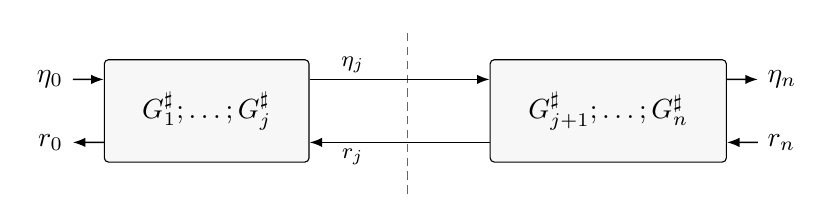
\begin{tikzpicture}[x=1cm,y=1cm]
        \node[figbox,minimum width=26mm,minimum height=13mm] (l) at (0,0) {$G_1^\sharp;\ldots;G_j^\sharp$};
        \node[figbox,minimum width=30mm,minimum height=13mm] (r) at (5.1,0) {$G_{j+1}^\sharp;\ldots;G_n^\sharp$};
        \draw[densely dashed,black!60] (2.55,-1.05)--(2.55,1.05);
        \node[anchor=east] (ein) at (-1.7,.40) {$\eta_0$};
        \node[anchor=east] (rout) at (-1.7,-.40) {$r_0$};
        \node[anchor=west] (eout) at (7,.40) {$\eta_n$};
        \node[anchor=west] (rin) at (7,-.40) {$r_n$};
        \draw[figwire] (ein)--([yshift=4mm]l.west);
        \draw[figwire] ([yshift=4mm]l.east)--node[figlabel,above,pos=.24] {$\eta_j$} ([yshift=4mm]r.west);
        \draw[figwire] ([yshift=4mm]r.east)--(eout);
        \draw[figwire] (rin)--([yshift=-4mm]r.east);
        \draw[figwire] ([yshift=-4mm]r.west)--node[figlabel,below,pos=.76] {$r_j$} ([yshift=-4mm]l.east);
        \draw[figwire] ([yshift=-4mm]l.west)--(rout);
    \end{tikzpicture}
    \caption{Cutting a serial chain after stage $j$. The prefix supplies $\eta_j$ to the suffix, and the suffix returns the whole table $r_j$. These are the boundary data for the induction, including rows at counterfactual inputs.}\label{fig:chain}
\end{figure}

\begin{theorem}[Serial evaluation]\label{thm:chain}
    For the constant host continuation $\kappa(\nu)=r_n$ and every bracketing of the encoded chain, the forward output is $\eta_n$, the backward output is the entire table $r_0$, and the profile passes exactly when
    \begin{equation}
        p_i\in E_i(x,v_i)\quad\text{for every }i
        \text{ and every }x\in\supp\eta_{i-1}.
        \label{eq:chain-test}
    \end{equation}
    For each $1\le i\le n+1$ and $x\in X_{i-1}$, the procedure $\mathsf{Return}(i,x)$ has law $r_{i-1}(x)$.
\end{theorem}
\begin{proof}\leavevmode
    \begin{enumerate}[titledsteps]
        \item \textbf{Evaluate a single stage.} For one box \eqref{eq:fwchain} and \eqref{eq:bwchain} are its play and coplay. Pulling the constant outer continuation through this box at a proposed input law $\eta'$ yields the table $C_i^\sharp(p_i,\eta',r_i)$. Equation~\eqref{eq:coplay} makes that table $r_{i-1}$ independently of $\eta'$. Hence the local continuation in the preceding box remains constant as a function of its forward law. At the box itself, point evaluation of the constant table gives precisely $v_i$ in \eqref{eq:common}.

        \item \textbf{Cut the chain.} For a cut after box $j$, the boundary data are $\eta_j$ and $r_j$. The right child takes $\eta_j$ on the forward pass and pulls its terminal table back to the constant continuation with value $r_j$. The left child then uses this continuation and the initial input. Applying the induction hypothesis to both children gives their common boundary data and all the local tests in \eqref{eq:chain-test}, whatever the cut.

        \item \textbf{Identify the sampled return law.} Write $Q_i(x)=\operatorname{Law}(\mathsf{Return}(i,x))$. The terminal clause gives $Q_{n+1}(x)=r_n(x)$. Conditioning on $a$ and applying the induction hypothesis gives
        \[
            \begin{aligned}
                Q_i(x)&=\sum_a p_i(a)\big(C_i(a,x,-)\big)_*Q_{i+1}(P_i(a,x))\\
                &=\sum_a p_i(a)\big(C_i(a,x,-)\big)_*r_i(P_i(a,x))
                =r_{i-1}(x).
            \end{aligned}
        \]
        The last equality is \eqref{eq:bwchain}. The procedure retains $a$ across the recursive call, so even strategies with the same play $P_i(a,x)$ use their own coplay.\qedhere
    \end{enumerate}
\end{proof}

For the games of Theorem~\ref{thm:reverse}, the return table gives the upstream player a strict preference for the risky action under either bracketing.

\begin{proof}[Evaluation of the sign example]
    In Theorem~\ref{thm:reverse}, the terminal return law at the output of $I$ is the point mass at $*$. At the input of $I$ the return row is $(\delta_{-1}+\delta_1)/2$, at either $y$. Its pushforward by $h_s$ is $\delta_{1/2}$, and its pushforward by $h_r$ is $\delta_1$. Equation~\eqref{eq:chain-test} therefore selects the risky action $r$ uniquely under either bracketing.
\end{proof}

A general host continuation can choose its terminal table as a function of the output law. To test a proposed output $y$ at stage $i$, we must therefore compute the law that the suffix would produce starting from $\delta_y$.

\begin{proposition}[Evaluation at an arbitrary host continuation]\label{prop:allcontexts}
    For fixed $p_i$, write $L_i$ for the forward operator in \eqref{eq:fwchain} and $B_i$ for the backward operator in \eqref{eq:bwchain}. Put $L_{>i}=L_n\circ\cdots\circ L_{i+1}$ and $B_{>i}=B_{i+1}\circ\cdots\circ B_n$. Empty composites are identities. For any host continuation $K$, the local test at stage $i$ is
    \[
        p_i\in E_i(x,v_i)\quad(x\in\supp\eta_{i-1}),\qquad
        v_i(y)=\alpha_{R_i}\!\left(
        \big[B_{>i}\big(K(L_{>i}(\delta_y))\big)\big](y)\right).
    \]
    The actual forward output is $\eta_n$ and the backward output against $K$ is $B_1\cdots B_n(K(\eta_n))$.
\end{proposition}
\begin{proof}
    At a proposed input law $\nu$ the ordinary host pullback of a continuation $K'$ through stage $j$ is $B_j(K'(L_j(\nu)))$, since \eqref{eq:coplay} is independent of the incoming law. Substitution through the suffix therefore gives the local continuation $\nu\mapsto B_{>i}(K(L_{>i}(\nu)))$. By \eqref{eq:flat}, evaluating this function at $\delta_y$ and taking the algebra value of its row at $y$ gives $v_i(y)$. The actual prefix supplies $\eta_{i-1}$, so \eqref{eq:common} gives exactly the displayed test.

    A cut composes the forward operators in play order and the backward operators in reverse order. Associativity of function composition makes both results independent of the cut. In particular, the actual output law is $\eta_n$ and the terminal table $K(\eta_n)$ pulls back to $B_1\cdots B_n(K(\eta_n))$.
\end{proof}

\begin{construction}[A decision separating two host continuations]
    Let an upstream decision choose between safe and risky. The downstream game has a single admissible lottery, a fair bit $b$. On the safe action the downstream game outputs $0$ and returns $1/2$ regardless of the payoff. On the risky action it outputs $b$ and passes the payoff back unchanged. Take both return types to be $\mathbb R$. Compare the host continuations
    \[
        K_0(\nu)(z)=\delta_0,\qquad
        K_1(\nu)(z)=\delta_{4\nu(0)\nu(1)} .
    \]

    They agree on every point law. At risky the downstream forward law is fair, so the local risky value is $0$ under $K_0$ and $1$ under $K_1$. The safe value is $1/2$ under either continuation. The prescribed downstream lottery passes at both inputs. Thus the whole chain distinguishes the two continuations even though their primitive point evaluations coincide.
\end{construction}

The example distinguishes continuations that agree on point laws. A related question concerns the return table itself. Could we replace each row by a statistic and still recover every upstream decision? Indicator payoffs show how a binary decision can detect a difference in a single row.

\begin{proposition}[Separation by backward tests]\label{prop:separate}
    Let $T$ be a set and $s:\D T\to W$ a statistic. If $\rho\mapsto\sum_t\rho(t)h(t)$ factors through $s$ for every $h:T\to\mathbb R$, then $s$ is injective. A strict binary decision distinguishes any two different return laws. The same holds for two return tables differing at any one row.
\end{proposition}
\begin{proof}\leavevmode
    \begin{enumerate}[titledsteps]
        \item \textbf{Separate return laws.} For each $t$ the expectation of $\mathbf{1}_{\{t\}}$ is $\rho(t)$. Thus $s(\rho)=s(\sigma)$ forces equality at every coordinate, whence $\rho=\sigma$. If $\rho$ and $\sigma$ differ at $t$, choose the constant safe payoff $c=(\rho(t)+\sigma(t))/2$. The expected indicator payoff is strictly above $c$ for one law and strictly below it for the other, giving opposite strict best replies.

        \item \textbf{Separate return tables.} More generally, let two tables differ at row $y_*$ and coordinate $t$, and choose $c$ from these two row probabilities. Use a binary upstream decision followed by a one-strategy game. On the test action this game plays $y_*$ and takes the indicator of the return. On safe it plays any fixed $y_0$ and returns $c$ regardless of the return. It always accepts. The two downstream tables give opposite unique best replies.

        For arbitrary return labels $T$, implement the test with the free backward algebra $\D T$ by pushing each table row along $z\mapsto\delta_z$. The test coplay $m\mapsto m(t)$ then has the desired expectation. When $y_0\ne y_*$, the test examines a row outside the path of the safe action.\qedhere
    \end{enumerate}
\end{proof}

\section{An associative serial rule on joint strategy laws}\label{sec:intrinsic}

The host encodes a profile as a tuple of lotteries, whereas GKLF test a joint law on the original pure strategies. To compare their equilibrium menus, we construct the associative composition directly on those joint laws. The construction uses two properties of the encoding. Continuation pullback composes along a chain, and the reachable inputs of a composite are the union of those reachable from its supported inputs.

\begin{construction}[Pullback of a continuation]
    Write $\mathsf T(X,S)=X\to\D S$ for the return tables and $\mathsf{Cont}(X,S)=\D X\to\mathsf T(X,S)$ for the continuations. For a game $G:(X,S)\to(Y,R)$ and a fixed lottery $p$, write $L_p^G:\D X\to\D Y$ and $B_p^G:\mathsf T(Y,R)\to\mathsf T(X,S)$ for \eqref{eq:play} and \eqref{eq:coplay}. A continuation $K\in\mathsf{Cont}(Y,R)$ pulls back to
    \[
        K^{G,p}=B_p^G\circ K\circ L_p^G\in\mathsf{Cont}(X,S).
    \]
\end{construction}

\begin{lemma}[Composition of the two passes]\label{lem:passes}
    Give $G;H$ its usual pure play and coplay. At the product lottery $p\otimes q$,
    \begin{align*}
        L_{p\otimes q}^{G;H}&=L_q^H\circ L_p^G,&
        B_{p\otimes q}^{G;H}&=B_p^G\circ B_q^H,&
        K^{G;H,p\otimes q}&=(K^{H,q})^{G,p}.
    \end{align*}
    The reachable set satisfies
    \begin{equation}
        \supp L_p^G\eta
        =\bigcup_{x\in\supp\eta}\supp L_p^G\delta_x .
        \label{eq:reach}
    \end{equation}
\end{lemma}
\begin{proof}
    For a point $x$ and strategies $a,b$, put $y_a=P_G(a,x)$ and $z_{ab}=P_H(b,y_a)$. Both forward expressions give $\sum_{a,b}p(a)q(b)\delta_{z_{ab}}$ at $\delta_x$ and extend by mixing over $x$. For $r\in\mathsf T(Z,T)$ both backward expressions at $x$ are
    \[
        \sum_{a,b}p(a)q(b)
        \bigl(t\mapsto C_G(a,x,C_H(b,y_a,t))\bigr)_* r(z_{ab}).
    \]
    Here the same $a,b$ occur on both passes. Substituting both operator identities into $B_{p\otimes q}^{G;H}\circ K\circ L_{p\otimes q}^{G;H}$ gives $(K^{H,q})^{G,p}$.

    For the support identity \eqref{eq:reach}, the mass at $y$ is $\sum_x\eta(x)(L_p^G\delta_x)(y)$. This finite sum is positive precisely when some $x\in\supp\eta$ contributes positive mass at $y$.
\end{proof}

Lemma~\ref{lem:passes} describes what reaches each game. To test a lottery at a mixed input we choose the $\D$-algebra on menus that intersects the sets of candidates with positive weight. Freeness of $\D X$ then gives a unique algebra-morphism extension of the \textbf{pointwise menu}.

\begin{construction}[Extending menus to input laws]\leavevmode
    \begin{enumerate}[titledsteps]
        \item \textbf{Extend a menu by intersection.} An arrow has the same pure data $(A,P_G,C_G)$ as before, together with a pointwise menu $M_G(x,K)\subseteq\D A$ for $K\in\mathsf{Cont}(Y,R)$. At an input law $\eta$, define
        \[
            \overline M_G(\eta,K)=\bigcap_{x\in\supp\eta}M_G(x,K).
        \]

        \item \textbf{Characterize the extension by its universal property.} For any $W$, give $\Pow W$ the algebra $\beta:\D(\Pow W)\to\Pow W$ that intersects the positive-weight sets. A Dirac law gives back its set. For a law of laws, both $\beta\mu$ and $\beta\D\beta$ intersect precisely the sets that occur with positive weight in a positive-weight inner law. The same support calculation also defines an algebra by union. The choice of intersection expresses the requirement that a candidate pass at every reachable input.

        For $T:X\to\Pow W$, its unique algebra-morphism extension to $(\Pow W,\beta)$ is
        \[
            T^\forall=\beta\circ\D T:\D X\longrightarrow\Pow W,\qquad
            T^\forall(\eta)=\bigcap_{x\in\supp\eta}T(x).
        \]
        Indeed $T^\forall\delta_X=T$. Any algebra morphism extending $T$ must send $\sum_x\eta(x)\delta_x$ to the intersection of the $T(x)$ of positive weight, which proves uniqueness.

        \item \textbf{Compose with an input kernel.} Testing at every reachable input also commutes with Kleisli composition. For a kernel $f:X\to\D Y$ and $T:Y\to\Pow W$, functoriality of $\D$ and $\beta\D\beta=\beta\mu$ give
        \[
            (T^\forall\circ f)^\forall
            =\beta\circ\D\beta\circ\D^2T\circ\D f
            =T^\forall\circ\mu_Y\circ\D f.
        \]
        Thus testing the same candidate along two successive kernels amounts to testing it along their Kleisli composite. With $W=\D A$ and $T(x)=M_G(x,K)$, this extension is exactly $\overline M_G(-,K)$.
    \end{enumerate}
\end{construction}

The two operations now specify a binary composition. The first game tests its lottery against the continuation pulled back through the second. The second tests its lottery at every input the first can produce.

\begin{construction}[Serial composition on joint strategy laws]
    Every original primitive gives such an arrow by $M_G(x,K)=E_G(x,y\mapsto\alpha_R(K(\delta_y)(y)))$. Give $G\diamond H$ ordinary serial play and coplay. At a point input $x$ put
    \begin{equation}
        M_{G\diamond H}(x,K)=
        \bigl\{p\otimes q\ \big|\ p\in M_G(x,K^{H,q}),\quad
        q\in\overline M_H(L_p^G\delta_x,K)\bigr\}.
        \label{eq:direct}
    \end{equation}
    The marginals of a proposed joint law are its only possible product factors. Thus the joint law determines both lotteries in the test.
\end{construction}

\begin{theorem}[Serial composition and comparison with the host]\label{thm:direct}
    The rule \eqref{eq:direct} defines a category on the original interface objects, modulo strategy bijections preserving the pure data and all pointwise menus. Its identity has one strategy, copies both interface values, and accepts its unique lottery. For any input law and continuation,
    \begin{equation}
        \overline M_{G\diamond H}(\eta,K)=
        \bigl\{p\otimes q\ \big|\ p\in\overline M_G(\eta,K^{H,q}),\quad
        q\in\overline M_H(L_p^G\eta,K)\bigr\}.
        \label{eq:direct-mixed}
    \end{equation}
    For a finite chain of original primitives with strategy sets $A_i$, the accepted joint laws are precisely the products $\bigotimes_i p_i$ for which $(p_i)_i$ is a host equilibrium. At each product profile, the forward operator $L_{\otimes_i p_i}$ of the direct composite equals the host play operator, and its backward operator $B_{\otimes_i p_i}$ equals the host coplay operator on return tables.
\end{theorem}
\begin{proof}\leavevmode
    \begin{enumerate}[titledsteps]
        \item \textbf{Compute the menu at a mixed input.} For $w\in\D(A\times B)$ take its marginals $p=(\pi_A)_*w$ and $q=(\pi_B)_*w$. Write $S=\supp\eta$ and $S_x=\supp(L_p^G\delta_x)$. Then
        \[
            \begin{aligned}
                &w\in\overline M_{G\diamond H}(\eta,K)\\
                \iff{}& w\in M_{G\diamond H}(x,K)\quad\text{for every }x\in S\\
                \iff{}& w=p\otimes q,\quad
                p\in\bigcap_{x\in S}M_G(x,K^{H,q}),\quad
                q\in\bigcap_{x\in S}\bigcap_{y\in S_x}M_H(y,K)\\
                \iff{}& w=p\otimes q,\quad
                p\in\overline M_G(\eta,K^{H,q}),\quad
                q\in\overline M_H(L_p^G\eta,K).
            \end{aligned}
        \]
        For the middle equivalence, $S$ is nonempty and every product decomposition of $w$ has factors $p,q$, so \eqref{eq:direct} uses these same marginals at every $x\in S$. The last equivalence uses $\bigcup_{x\in S}S_x=\supp(L_p^G\eta)$ from \eqref{eq:reach}. This proves \eqref{eq:direct-mixed}.

        \item \textbf{Prove associativity and the unit equations.} Take a third arrow $I$ and lotteries $p,q,s$. In either bracketing every accepted law factors as $p\otimes q\otimes s$. For the left bracketing, apply \eqref{eq:direct-mixed} to the first two factors. In the right bracketing apply it to the final two factors at the intermediate law $L_p^G\eta$. For such a product the three tests in both bracketings are
        \begin{align*}
            p&\in\overline M_G\bigl(\eta,(K^{I,s})^{H,q}\bigr),\\
            q&\in\overline M_H\bigl(L_p^G\eta,K^{I,s}\bigr),\\
            s&\in\overline M_I\bigl(L_q^H L_p^G\eta,K\bigr).
        \end{align*}
        Lemma~\ref{lem:passes} identifies the pulled-back continuation and the twice-propagated input in the two expansions. This proves associativity on the entire joint-law space.

        For the identity, $L$ and $B$ are identity functions, $K^{\mathrm{id},*}=K$, and its sole local test passes. Formula~\eqref{eq:direct-mixed} gives each unit equation under the singleton strategy bijection. A relabelling of strategies pushes each lottery to its renamed marginal, preserves $L,B$ by reindexing finite sums, and carries products to products. Composition therefore descends to the indicated equivalence classes.

        \item \textbf{Identify the host equilibria.} For a primitive, $\overline M_G$ is exactly \eqref{eq:common}. Under ordinary host composition the first factor sees $(\eta,K^{H,q})$ and the second sees $(L_p^G\eta,K)$. This is precisely \eqref{eq:direct-mixed} under the injection $(p,q)\mapsto p\otimes q$. Induct on a cut of the chain and use Lemma~\ref{lem:passes} for the play, coplay and continuation of each child. This gives the claimed equality of equilibrium menus after readout for every $\eta,K$ and every cut.

        A host profile is a tuple of lotteries $(p_i)_i$. The corresponding equilibrium of the direct composite is the single law $\bigotimes_i p_i$ on tuples of original pure strategies.\qedhere
    \end{enumerate}
\end{proof}

\subsection{Which GKLF bracketings contain every equilibrium?}

For two games, Proposition~\ref{prop:two} shows that GKLF accept every joint law admitted by the associative rule. Theorem~\ref{thm:direct} lets us ask which bracketings preserve this inclusion along a longer chain. For an ordered binary bracketing $T$ of $n\geq1$ primitives, let $E_T(x,k)$ be its GKLF menu at an ordinary point context, and let $M(x,\kappa_k)$ be the menu of the associative rule. Both menus are sets of laws on the same strategy tuples under the canonical reassociation.

\begin{theorem}[Characterization of the right-associated bracketing]\label{thm:comb}
    For a fixed bracketing $T$, the inclusion
    \[
        M(x,\kappa_k)\ \subseteq\ E_T(x,k)
    \]
    holds for all choices of primitives and ordinary point contexts if and only if $T$ is fully right-associated. For every $T$, the two menus agree on all point masses on strategy tuples.
\end{theorem}

At each cut of a fully right-associated tree the left child is a single game. The downstream test at that cut can use one equilibrium lottery for the entire suffix.

\begin{proof}\leavevmode
    \begin{enumerate}[titledsteps]
        \item \textbf{Inclusion for the fully right-associated bracketing.} Fix an equilibrium $(p_1,\ldots,p_n)$ of the associative rule and write $w_i=\bigotimes_{j=i}^n p_j$ for the joint lottery on the suffix beginning at $i$. Start the forward recursion \eqref{eq:fwchain} at $\eta_0=\delta_x$ and the backward recursion \eqref{eq:bwchain} at $r_n(z)=\delta_{k(z)}$. We claim that the right-associated GKLF suffix beginning at $i$ accepts $w_i$ at every $x'\in\supp\eta_{i-1}$ with continuation $k$. At $i=n$ this is the primitive equilibrium test, since $\alpha_{R_n}r_n=k$.

        Suppose the claim holds for the suffix beginning at $i+1$. For any proposed output $y$ of $G_i$, the pure suffix plays forward from $y$, applies $k$, and returns through the same tuple of pure strategies. Sampling that tuple under $w_{i+1}$ gives $r_i(y)$ by Theorem~\ref{thm:chain}. Thus the GKLF upstream continuation is $y\mapsto\alpha_{R_i}r_i(y)$, against which $p_i$ passes at $x'$ by \eqref{eq:chain-test}.

        The downstream input law $L_{p_i}^{G_i}\delta_{x'}$ has support contained in $\supp\eta_i$ by \eqref{eq:reach}. The induction hypothesis puts the same $w_{i+1}$ in the menu at every one of those inputs. Using it in every row witnesses the downstream lift by Lemma~\ref{lem:lift}. The two tests admit $p_i\otimes w_{i+1}=w_i$. Taking $i=1$ proves inclusion at the root. Proposition~\ref{prop:two} shows that inclusion can already be strict for two leaves.

        \item \textbf{A counterexample for every other bracketing.} Any other tree has an internal node whose left child is itself internal. Mark one leaf in each branch of that left child and one leaf in the right child of the chosen node. In order of play, put the games $G,H,I$ of Theorem~\ref{thm:reverse} at the marked leaves and the appropriate interface identity at every other leaf. The marked leaves induce the bracketing $(G;H);I$.

        To erase the other leaves under the GKLF rule, first contract each subtree consisting entirely of identities. Its unique strategy copies play and coplay and passes every test, so this is an identity up to the unique strategy bijection. At a node with only one marked side, an output identity erases, whereas an input identity takes the convex hull of the remaining menu by Proposition~\ref{prop:unit}. It therefore suffices to check convexity for every reduced subtree containing a mark.

        Each of $G,H,I$ has convex menus in every context. For $G;H$, the menu at a continuation $k'$ consists of the maximizers of the linear functional $p\mapsto\sum_y p(y)h_y(k'(y))$ paired with the unique middle strategy, and is again convex. The only remaining reduced subtree is $(G;H);I$, whose menu is a singleton at its sole context by Theorem~\ref{thm:reverse}. Induction from the leaves now shows that erasure preserves play, coplay and every menu.

        The reduced GKLF game selects the safe action. Identities also erase under the associative rule by Theorem~\ref{thm:direct}, and the sign calculation following Theorem~\ref{thm:chain} selects the risky action. Its equilibrium therefore witnesses the failure of inclusion for the chosen tree.

        \item \textbf{Agreement on pure profiles.} For $N\subseteq\D A$, one has $\delta_a\in\conv N$ exactly when $\delta_a\in N$, since every positive-weight term in a convex combination equal to $\delta_a$ must itself be $\delta_a$. At a pure profile the forward law at each cut is a point mass. Lemma~\ref{lem:lift} and this extremality reduce the GKLF downstream test to membership in the menu at the single reached input, which is also the downstream test of the associative rule.

        Upstream, a pure suffix sends each deterministic return row to a deterministic row. The associative rule thus pulls back a constant deterministic table whose value at each proposed output is the pure suffix coplay. Averaging that pure coplay in the GKLF rule gives exactly the same continuation. Induction on the two children of each cut reduces both predicates to identical tests at the primitive leaves.\qedhere
    \end{enumerate}
\end{proof}

The uniqueness in Theorem~\ref{thm:comb} is uniform over interface types as well as over games. For example, if all interfaces are $(\one,\one)$, every bracketing contains every equilibrium of the associative rule for arbitrary primitive menus. At a leaf the menus agree. At each cut, the accepted product factors for the associative rule belong to the two child menus by induction, and \eqref{eq:star} admits their product since $N\subseteq\conv N$ for the right child's menu $N$.

\section{Independent states and shared observations}\label{sec:signals}

The classification concerns joint laws of strategies. A different kind of dependence arises when players with independently chosen policies observe the same signal. In Aumann's formulation, a random device can correlate players' actions through the information they receive \cite{aumann}. For the indifferent games $U_A^\sharp,U_B^\sharp,U_C^\sharp$, every triple of lotteries $(p,q,r)$ is an equilibrium and has the same independent joint law $p\otimes q\otimes r$ under both bracketings. The law $u\otimes d$ of Theorem~\ref{thm:assoc} can nevertheless be realized on the players' \textbf{actions} by giving the last two players a common observation.

\begin{construction}[A shared observation]\leavevmode
    \begin{enumerate}[titledsteps]
        \item \textbf{Supply a common observation.} In the Markov category $\Kl(\D)$, write $U=\{0,1\}$ and regard the fair law as a state $u:\one\to U$. The copy map $\Delta_U:U\to U\times U$ is the deterministic diagonal, viewed as a kernel \cite{fritz}. The states $u\otimes u$ and $\Delta_U\circ u$ describe two different experiments (Figure~\ref{fig:signal}). In the second, a device draws $s$ once and both agents observe it.

        \item \textbf{Compute the induced action law.} Give them deterministic policies $b(s)=s=c(s)$ and constant payoffs. Use a single joint observation port with input law $u$ and the deterministic map $s\mapsto(b(s),c(s))$ in \eqref{eq:play}. Inside this deterministic map the diagonal $s\mapsto(s,s)$ supplies the same realized bit to both response functions. Taking the pushforward after this copy gives the joint action law. For the two identity policies this law is $d$. An independent first player gives the action law $u\otimes d$. The response policies are deterministic throughout. Dependence of the actions arises from the observation wire.
    \end{enumerate}
\end{construction}

\begin{figure}[!htbp]
    \centering\small
    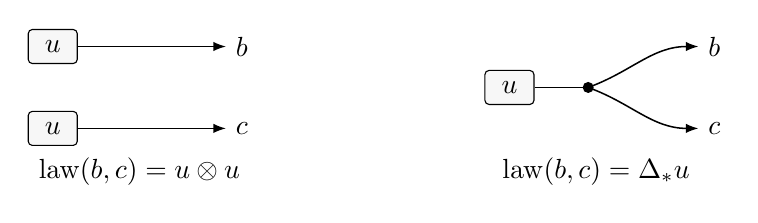
\begin{tikzpicture}[x=1cm,y=1cm]
        \begin{scope}
            \node[figbox] (u1) at (0,.52) {$u$};
            \node[figbox] (u2) at (0,-.52) {$u$};
            \draw[figwire] (u1)--(2.2,.52) node[right] {$b$};
            \draw[figwire] (u2)--(2.2,-.52) node[right] {$c$};
            \node at (1.1,-1.07) {$\operatorname{law}(b,c)=u\otimes u$};
        \end{scope}
        \begin{scope}[xshift=5.8cm]
            \node[figbox] (u) at (0,0) {$u$}; \coordinate (d) at (1,0);
            \draw[line width=.55pt] (u)--(d);
            \draw[figwire] (d) to[out=20,in=180] (2.4,.52) node[right] {$b$};
            \draw[figwire] (d) to[out=-20,in=180] (2.4,-.52) node[right] {$c$};
            \fill (d) circle (2pt);
            \node at (1.1,-1.07) {$\operatorname{law}(b,c)=\Delta_*u$};
        \end{scope}
    \end{tikzpicture}
    \caption{Each $u$ box samples one fresh bit. The dot copies the sampled value by $\Delta(s)=(s,s)$. The left circuit gives mass $1/4$ to $(0,1)$. The right gives mass zero.}\label{fig:signal}
\end{figure}

A shared input explains correlated actions. For two independently sampled ports the remaining question is how to evaluate a payoff that depends on both outputs. The following lens combines the input laws and returns to each port its payoff averaged over the other.

\begin{construction}[The \textbf{independent-port comparison}]\leavevmode
    \begin{enumerate}[titledsteps]
        \item \textbf{Combine the forward states.} For two interfaces write $J:F(X_1,S_1)\otimes F(X_2,S_2)\to F(X_1\times X_2,S_1\times S_2)$ for the following comparison lens in the ambient category of ordinary open games. As a host game it has one strategy and always accepts. Its play sends $(\eta_1,\eta_2)$ to $\eta_1\otimes\eta_2$.

        \item \textbf{Project the joint return.} On a return table $r$ its two coplay rows are
        \begin{align}
            J_1(\eta_2,r)(x_1)
            &=\sum_{x_2}\eta_2(x_2)(\pi_1)_*r(x_1,x_2),\nonumber\\
            J_2(\eta_1,r)(x_2)
            &=\sum_{x_1}\eta_1(x_1)(\pi_2)_*r(x_1,x_2).
            \label{eq:bundle}
        \end{align}
        The first component averages over the second input law, and conversely for the second component. Appendix~\ref{app:optic} proves the coherence of this comparison and its naturality for stochastic lenses at fixed profiles.
    \end{enumerate}
\end{construction}

The two backward components have a categorical description in terms of the partial effects used by the Nash product of Capucci, Gavranovi\'{c}, Hedges and Rischel \cite[Proposition~14]{capucci}. For states $s_i:I\to U_i$ and an effect $e:U_1\otimes U_2\to I$, these partial effects are, up to unitors,
\[
    e\circ(1_{U_1}\otimes s_2),\qquad
    e\circ(s_1\otimes 1_{U_2}).
\]
Under \eqref{eq:state-effect}, let $s_i$ correspond to the input law $\eta_i$ and $e$ to the return table $r$. The first partial effect supplies $x_2\sim\eta_2$ and discards the second backward coordinate. At $x_1$ this gives exactly $J_1(\eta_2,r)(x_1)$ in \eqref{eq:bundle}. The second gives $J_2(\eta_1,r)$ in the same way. The lens $J$ packages these two partial effects together with the independent product of the forward states.

For determinised games, GKLF compare the tensor of the determinisations with the determinisation of the tensor at a Kleisli-extended payoff, using independent product and marginal projections \cite[Lemma~9]{gklf}. In our encoding the backward values are whole tables. The lens $J$ supplies a table at each port by \eqref{eq:bundle}.

\begin{proposition}[Parallel comparison at an ordinary context]\label{prop:tensor}
    Let $G_1,G_2$ be any two original games, let $(x_1,x_2)$ be a point input, and let $k:Y_1\times Y_2\to R_1\times R_2$ be any payoff. The host tensor of their encodings, observed through $J$ and $\kappa_k$, accepts $(p_1,p_2)$ exactly when the GKLF tensor accepts $p_1\otimes p_2$ at $((x_1,x_2),k)$. All accepted laws of that tensor arise uniquely in this way.
\end{proposition}
\begin{proof}
    At output laws $(\nu_1,\nu_2)$ the pullback of $\kappa_k$ through $J$ gives the two tables
    \[
        y_1\mapsto (\pi_1 k(y_1,-))_*\nu_2,\qquad
        y_2\mapsto (\pi_2 k(-,y_2))_*\nu_1 .
    \]
    Indeed substitute $r(y_1,y_2)=\delta_{k(y_1,y_2)}$ in \eqref{eq:bundle}.

    The host tensor fixes the opponent's actual $\nu_j=(P_j(-,x_j))_*p_j$ when testing a deviation. At $\delta_{y_i}$, extracting row $y_i$ and applying $\alpha_{R_i}$ gives the GKLF continuation against the opponent's lottery. The input is a point, hence the two local menus are exactly those in \cite[Definition~5]{gklf}. The definition admits only product laws, and their marginals recover $p_1,p_2$.
\end{proof}

Hedges computes the tensor of stochastic decisions by playing a tuple of strategy lotteries as its independent product and testing each decision against the opponents' lotteries \cite[Sections~3.1.6--3.1.7]{hedges}. Matching pennies illustrates this test in Proposition~\ref{prop:tensor} and distinguishes it from a predicate on the marginals of an arbitrary joint law.

\begin{construction}[Matching pennies]\leavevmode
    \begin{enumerate}[titledsteps]
        \item \textbf{Form the two-player game.} Use the two decision primitives of \cite[Example~6]{gklf}. Each has type $(\one,\mathbb R)\to(\{0,1\},\mathbb R)$, plays its strategy bit and passes the payoff back unchanged. Against $v:\{0,1\}\to\mathbb R$, its menu is the argmax of $\sum_y p(y)v(y)$ over all lotteries $p$. Let the external payoff be $(k_1,k_2)$, where $k_1(y,z)$ is $+1$ at agreement and $-1$ otherwise, and $k_2=-k_1$. Define the host continuation at the two ports by
        \[
            \kappa(\nu_1,\nu_2)=
            \left(y\mapsto(k_1(y,-))_*\nu_2,\quad
            z\mapsto(k_2(-,z))_*\nu_1\right).
        \]
        The local continuation for the first decision fixes the second forward law, and conversely for the second decision. Evaluation by \eqref{eq:flat}, with $\alpha_{\mathbb R}$ ordinary expectation, gives the expected payoff of each pure alternative against the other player.

        \item \textbf{Solve the two best-response conditions.} If $p$ and $q$ are the two probabilities of playing $1$, the expected first payoff is $(2p-1)(2q-1)$. If $q>1/2$, the first player strictly prefers $p=1$, in which case the second strictly prefers $q=0$. If $q<1/2$, the first strictly prefers $p=0$, to which the second replies $q=1$. At $q=1/2$ the first is indifferent, and an interior $q$ is a best reply for the second precisely at $p=1/2$. The unique accepted pair is $(u,u)$, with joint law $u\otimes u$. This agrees with the tensor rule of \cite[Definition~5 and Example~6]{gklf}.

        \item \textbf{Compare with the marginal test.} The stand-alone predicate in \cite[Example~4]{gklf} tests only the marginals. In the order $00,01,10,11$, its entire menu consists of the laws
        \[
            (t,\,1/2-t,\,1/2-t,\,t),\qquad 0\le t\le 1/2 .
        \]
        Indeed the row and column sums must be $1/2$, which determines the last three entries from the first. The product occurs at $t=1/4$ and the diagonal law $d$ at $t=1/2$.

        Example~6 of \cite{gklf} identifies the tensor with the stand-alone game of Example~4. At this payoff the tensor menu is a singleton and the stand-alone menu is the entire displayed family. A strategy bijection induces a bijection on laws, so no strategy bijection can identify those menus. The diagonal coupling also fails the incentive test for a correlated equilibrium \cite{aumann}. Given the common bit as a recommendation, the second player gains by flipping it.
    \end{enumerate}
\end{construction}

\section{Comparison with determinisation and stochastic semantics}\label{sec:related}

The use of a lottery as a pure strategy of an ordinary game already appears in GKLF's determinisation $\Delta G:(X,S)\to(\D Y,\D R)$. Given $k:Y\to R$, the continuation $\D k:\D Y\to\D R$ recovers the primitive equilibrium test because $\alpha_R\circ\D k\circ\delta_Y=k$ \cite[Definition~7 and Lemma~8]{gklf}. Their variant $\Delta' G:(\D X,\D S)\to(\D Y,\D R)$ also takes a law on inputs and uses the downstream lift $\D^\#$ \cite[Proposition~20]{gklf}. That result treats morphisms between games. In the same setting their right adjoint $\Psi$ assigns the pure menu $\{a\mid\delta_a\in E_G(x,k)\}$ \cite[Theorem~21]{gklf}.

Theorem~\ref{thm:comb} compares these Dirac verdicts across serial bracketings. For general lotteries, our encoding retains a separate return law at each possible input and intersects the reachable equilibrium menus. Proposition~\ref{prop:two} compares the resulting serial test with GKLF's.

Atkey et al.\ propose to recover GKLF serial composition from a graded bimodule \cite[Theorem~29 and Example~37]{atkey}. Appendix~E.1, Lemma~51, of their extended version gives the left action $\ell_{J,K}$ explicitly \cite{atkeyext}.

\begin{proof}[Unit comparison]
    Put the identity lens in the first slot of this action and identify $\one\times B$ with $B$. A candidate $q\in\D B$ corresponds to $\delta_*\otimes q$, so the action's product condition holds. Identity play sends $x$ to $\delta_x$ under the sole strategy lottery. Writing $E$ for the menu in the second slot, the displayed left action therefore accepts $q$ exactly when
    \[
        q\in\D^\#\bigl(y\mapsto E(y,k)\bigr)(\delta_x)
        =\conv E(x,k).
    \]
    For the binary menu $E(x,k)=\{\delta_0,\delta_1\}$ this action admits the fair lottery. The left unit equation requires the original two-element menu. Hence the proposed probabilistic action in Lemma~51 fails the left unit equation on unrestricted GKLF menus. The graded-bimodule construction in their Theorem~29 requires this equation for its application to Example~37.
\end{proof}

The convexification in this unit test has an algebraic explanation. Goy and Petri\c{s}an identify convex hull as the idempotent defining the convex powerset in the weak lifting \cite[Theorem~4.1]{goy}. At a game interface, the same operation can enlarge even the image of two full strategy simplices under independent product. The diagonal law in Theorem~\ref{thm:assoc} exhibits the resulting change in the players' randomization.

Bolt, Hedges and Zahn model Bayesian open games in environments where an external variable can correlate a state with a continuation \cite[Definition~3.5.2]{bolt}. They prove associativity for their open games by composing the local contexts \cite[Lemma~3.10.1]{bolt}. Their Bayesian agent tests a behavioural policy at every observation of positive probability using the posterior expected payoff \cite[Definition~4.4.1]{bolt}. The evaluation map following Definition~\ref{def:encode} identifies the corresponding test on policy lotteries when the latent state is a singleton. For general primitives our equilibrium test retains the same lottery across the reachable menus.

In his treatment of open games in stochastic modules, Rischel distinguishes random selection of a strategy from random play specified by the strategy, and explains how deterministic selection of stochastic policies gives a tensor profile with separate strategy coordinates \cite[Section~5.2, p.~78]{rischel}. Our comparison in Theorem~\ref{thm:direct} reads a tuple of primitive lotteries back as a law on the original pure strategy tuples. For the process determined by a fixed strategy lottery, the following stochastic lens retains the dependence between play and coplay.

\begin{construction}[A residual for a fixed strategy lottery]
    For a fixed lottery $p$ on $A$, take $M=X\times A$ as residual in the coend of \cite[Definition~3.3.1]{bolt}. Keep the sampled $a$ together with $x$ and output the play,
    \[
        x\longmapsto\sum_a p(a)\delta_{((x,a),P(a,x))}.
    \]
    Use the retained pair to return the coplay,
    \[
        ((x,a),t)\longmapsto\delta_{C(a,x,t)}.
    \]
    Figure~\ref{fig:residual} displays the retained pair in this representative.
\end{construction}

\begin{figure}[!htbp]
    \centering\small
    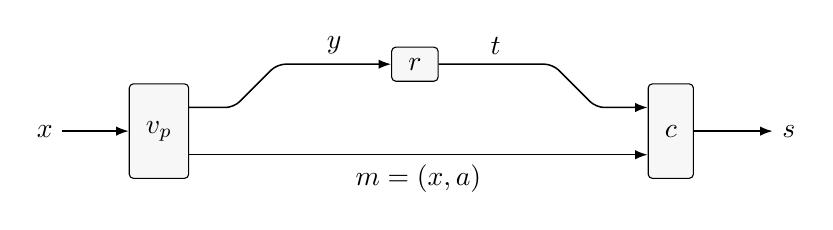
\begin{tikzpicture}[x=1cm,y=1cm]
        \node (x) at (-1.45,0) {$x$};
        \node[figbox,minimum height=12mm] (v) at (0,0) {$v_p$};
        \node[figbox] (r) at (3.25,.85) {$r$};
        \node[figbox,minimum height=12mm] (c) at (6.5,0) {$c$};
        \node (s) at (8,0) {$s$};
        \draw[figwire] (x)--(v); \draw[figwire] (c)--(s);
        \draw[figwire,rounded corners=3pt] ([yshift=3mm]v.east)--(.95,.30)--(1.5,.85)--node[above] {$y$} (r);
        \draw[figwire,rounded corners=3pt] (r)--node[above] {$t$} (5,.85)--(5.55,.30)--([yshift=3mm]c.west);
        \draw[figwire] ([yshift=-3mm]v.east)--node[below] {$m=(x,a)$} ([yshift=-3mm]c.west);
    \end{tikzpicture}
    \caption{Residual wire of the fixed-profile stochastic lens. The forward kernel $v_p$ draws $a$ and produces $(m,y)$. The final kernel $c$ uses the retained $m$ and the sampled return $t$ to output $C(a,x,t)$.}\label{fig:residual}
\end{figure}

Composing this representative with a state gives the forward law \eqref{eq:play}. Composing it with an effect gives the backward table \eqref{eq:coplay}. Proposition~\ref{prop:optic} shows that both computations respect the coend relation and that their actions on independent ports form a lax symmetric monoidal functor. The stochastic lens thus determines the process at a fixed lottery. The primitive equilibrium menus determine which lotteries the game admits.

\section*{Conclusion}

A player evaluating a deviation may need a return at an output that the actual play never reaches. Retaining the whole return table makes that comparison possible, even for a nonlinear coplay. On the forward pass, the reachable inputs determine where a lottery must be admissible. Requiring the same lottery across those inputs preserves its identity as a factor of the joint strategy law whenever the sequence is cut.

At an ordinary point context, the host composite $(G_1^\sharp\otimes G_2^\sharp);J$ recovers exactly the GKLF tensor menu under independent readout. For serial composition on joint laws, only full right association guarantees that the GKLF menu contains every equilibrium of the associative rule. An input-dependent witness can already make that inclusion strict for two games. Correlated actions remain possible in either setting when the wiring specifies a shared observation.

\appendix

\section{Computing the host contexts}\label{app:host}

The encoding uses ordinary open-game composition. We record the contexts that this composition passes to a component, first in a chain and then across a tensor. These formulas account for the local tests in Theorem~\ref{thm:chain} and Proposition~\ref{prop:tensor}.

\begin{proof}[Serial context calculation]
    For ordinary games $G,H$ with fixed strategies $a,b$, put $y=P_G(a,x)$. The serial equilibrium conditions are
    \[
        a\in E_G(x,y'\mapsto C_H(b,y',k(P_H(b,y')))),\qquad
        b\in E_H(y,k).
    \]

    Play and coplay compose as in Section~\ref{sec:rule}. To check associativity directly, append a game $I$ with strategy $c$. The continuation for the first game at a proposed $y'$ becomes, in both bracketings,
    \[
        C_H\bigl(b,y',C_I(c,P_H(b,y'),k(P_I(c,P_H(b,y'))))\bigr).
    \]
    The second game receives $y$ and the continuation pulled back through $I$ alone. The third receives $P_H(b,y)$ and the outer continuation. Thus each required membership has identical arguments on both sides. With an identity, pullback gives $y'\mapsto k(y')$, and the identity's other test always passes.
\end{proof}

\begin{proof}[Tensor context calculation]
    For the host tensor, write $y_i=P_i(a_i,x_i)$ and let the outer continuation be $K$. The component continuations are $y\mapsto\pi_1 K(y,y_2)$ and $z\mapsto\pi_2 K(y_1,z)$. Pairing the play and coplay maps componentwise therefore leaves precisely these two local equilibrium tests.

    For the encoded games each $y_i$ here is itself a law and each projected return is a whole table. These expressions give the continuations used in matching pennies. Reassociating or permuting product ports changes their tuple coordinates by the canonical bijections. The serial and tensor formulas are also the fixed-point formulas for the diagonal best-response relations used in Theorem~\ref{thm:rep}.
\end{proof}

\section{States and effects of stochastic lenses}\label{app:optic}

At a fixed strategy lottery, Section~\ref{sec:related} identified play and coplay with the action of a stochastic lens on states and effects. Here we verify that this action respects the coend relation and prove coherence of the comparison lens $J$ for independent ports.

Write $\Opt=\mathrm{Lens}_{\mathcal K}$ for coend lenses over $\mathcal K=\Kl(\D)$, and $\mathrm{Lens}_{\Set}$ for ordinary set-based lenses. For $U=(X,S)$ and $V=(Y,R)$, the hom-set is the coend
\[
    \Opt(U,V)=\int^{M\in\mathcal K}
    \mathcal K(X,M\otimes Y)\times\mathcal K(M\otimes R,S).
\]
A representative $(M,v,u)$ thus consists of a residual and kernels $v:X\to\D(M\times Y)$, $u:M\times R\to\D S$. The coend identifies applying a residual kernel to the output of the forward leg with applying it to the input of the backward leg \cite[Definition~3.3.1]{bolt}.

\begin{construction}[The underlying state-and-effect functor]
    Using \eqref{eq:state-effect}, the underlying functor of the following proposition is the composite
    \[
        \Opt\xrightarrow{\ (\St,\Ef)\ }\Set\times\Set^{\mathrm{op}}
        \xrightarrow{\ \iota\ }\mathrm{Lens}_{\Set}.
    \]
    Here $\iota(f,g)$ has play $f$ and coplay $(x,r)\mapsto g(r)$, as in \cite[Section~5]{gklf}. A lens $\ell:U\to V$ acts by $\eta\mapsto\ell\circ\eta$ on states and by $r\mapsto r\circ\ell$ on effects. Formula~\eqref{eq:optic} computes these two actions on representatives.

    The tensor comparison is the lens $J$ of \eqref{eq:bundle}. Its backward component averages each projected return against the state at the other port.
\end{construction}

\begin{proposition}[States, effects and independent tensor ports]\label{prop:optic}
    There is a lax symmetric monoidal functor from stochastic coend lenses to ordinary set-based lenses with object map $F$. On a representative $(M,v,u)$ its forward and backward operators are
    \begin{align}
        (L\eta)(y)&=\sum_{x,m}\eta(x)v(x)(m,y),\nonumber\\
        (Br)(x)&=\sum_{m,y,t}v(x)(m,y)r(y)(t)\,u(m,t).
        \label{eq:optic}
    \end{align}
    The backward leg of the ordinary lens returns $Br$ at every input law. The tensor comparison is $J$ from \eqref{eq:bundle} and the unit comparison is the canonical map between singleton interfaces.
\end{proposition}
\begin{proof}\leavevmode
    \begin{enumerate}[titledsteps]
        \item \textbf{Compute the actions and descend to the coend.} Composing a state $\eta$ with $(M,v,u)$ discards the residual and gives the $Y$-marginal of $v$ averaged over $\eta$. Composing $(M,v,u)$ with an effect $r$ draws $(m,y)$ from $v(x)$, applies $r$ at $y$, and then applies $u(m,-)$. This yields \eqref{eq:optic}. All sums have finite support at the given input or row. Total mass is one by summing the kernels from last to first.

        For a residual kernel $d:M\to\D N$ and a backward leg $u':N\times R\to\D S$, sliding $d$ forward or backward gives the same expression
        \[
            \sum_{m,n,y,t} v(x)(m,y)d(m)(n)r(y)(t)\,u'(n,t).
        \]
        The forward marginal is unchanged because $\sum_n d(m)(n)=1$. Hence \eqref{eq:optic} respects each generating coend relation.

        \item \textbf{Verify functoriality.} The singleton-residual identity gives the identity operators. For composable lenses, write the second representative as $(N,v',u')$. The composite retains $(m,n)$, chooses $(m,y)$ under $v(x)$, then $(n,z)$ under $v'(y)$, and passes the return first through $u'$ and then through $u$ \cite[Definition~3.3.4]{bolt}. Its forward projection is $L'L$. Given a terminal table $r$, its backward row is
        \[
            \sum_{m,y,n,z,t,b}v(x)(m,y)v'(y)(n,z)r(z)(t)u'(n,t)(b)\,u(m,b)
            =\bigl(B(B'r)\bigr)(x).
        \]
        These are the ordinary lens composition formulas.

        \item \textbf{Check the monoidal coherence diagrams.} To check coherence, identify rebracketed or permuted tuples by their canonical bijections. Formula~\eqref{eq:optic} pushes the input law forward along each such bijection and reindexes both the arguments and the return coordinates of the backward table. For the tensor comparison, both parenthesizations of three instances of \eqref{eq:bundle} produce the forward law $\eta_1\otimes\eta_2\otimes\eta_3$. In the first backward component both give, at $x_1$,
        \[
            \sum_{x_2,x_3}\eta_2(x_2)\eta_3(x_3)(\pi_1)_*r(x_1,x_2,x_3).
        \]
        The other two components follow by the corresponding coordinate projections.

        A singleton factor contributes its unique mass one and its unique backward row. Interchanging the two ports interchanges the two sums in \eqref{eq:bundle}, giving the symmetry diagram. This verifies the associativity, unit and symmetry conditions.

        \item \textbf{Prove naturality of the tensor comparison.} For naturality take representatives $(M_i,v_i,u_i)$ for two lenses. Write $\nu_i=L_i\eta_i$ and let $r$ be a joint output table. Combining the two lenses first and then applying $J$ gives at $x_1$ the first backward row
        \[
            \sum_{m,y,z,t}v_1(x_1)(m,y)\nu_2(z)
            \big[(\pi_1)_*r(y,z)\big](t)\,u_1(m,t).
        \]

        On the other route, first form the product input at $J$ and apply \eqref{eq:optic} to the tensor representative. The first projected backward law at $(x_1,x_2)$ integrates out the second backward kernel, whose total mass is one. Averaging this law over $x_2$ sums the second forward kernel to $\sum_{x_2,m_2}\eta_2(x_2)v_2(x_2)(m_2,z)=\nu_2(z)$, giving the same displayed expression. Projection to the second component gives the corresponding equality with the indices exchanged. The forward equality is $L_{1\otimes2}(\eta_1\otimes\eta_2)=\nu_1\otimes\nu_2$ by independence. This proves the naturality square for ordinary lenses.\qedhere
    \end{enumerate}
\end{proof}

For the representative with $M=X\times A$ in Section~\ref{sec:related}, substituting its two kernels into \eqref{eq:optic} gives \eqref{eq:play} and \eqref{eq:coplay} term by term. Proposition~\ref{prop:optic} therefore compares the passes of any composite of fixed profiles. Equilibrium for variable profiles enters separately through the primitive menus, as in Theorem~\ref{thm:direct} and Proposition~\ref{prop:tensor}.

\section*{Statements and Declarations}

\noindent\textbf{Funding.} The author received no funding for this research.

\smallskip
\noindent\textbf{Competing interests.} The author declares no competing interests.

\smallskip
\noindent\textbf{Author contributions.} The sole author carried out the research and prepared the manuscript.

\smallskip
\noindent\textbf{Data availability.} This article presents theoretical results. No datasets were generated or analysed.

\smallskip
\noindent\textbf{Use of AI-assisted tools.} Generative AI systems were used during the research and development of this manuscript. Responsibility for the mathematical content, arguments, and conclusions rests with the author.

\begin{thebibliography}{99}

    \bibitem{atkeyext}
    Robert Atkey, Bruno Gavranovi{\'c}, Neil Ghani, Clemens Kupke, J{\'e}r{\'e}my Ledent, and Fredrik {Nordvall Forsberg}. \newblock Compositional game theory, compositionally. \newblock Extended version for Applied Category Theory 2020, Appendix~E.1. \url{https://fredriknf.com/papers/compcgt_act2020.pdf}.

    \bibitem{atkey}
    Robert Atkey, Bruno Gavranovi{\'c}, Neil Ghani, Clemens Kupke, J{\'e}r{\'e}my Ledent, and Fredrik {Nordvall Forsberg}. \newblock Compositional game theory, compositionally. \newblock {\em Electronic Proceedings in Theoretical Computer Science}, 333:198--214, 2021. \newblock \url{https://doi.org/10.4204/EPTCS.333.14}.

    \bibitem{aumann}
    Robert J. Aumann. \newblock Subjectivity and correlation in randomized strategies. \newblock {\em Journal of Mathematical Economics}, 1(1):67--96, 1974. \newblock \url{https://doi.org/10.1016/0304-4068(74)90037-8}.

    \bibitem{barr}
    Michael Barr. \newblock Relational algebras. \newblock In {\em Reports of the Midwest Category Seminar~IV}, volume 137 of Lecture Notes in Mathematics, pages 39--55. Springer, 1970. \newblock \url{https://doi.org/10.1007/BFb0060439}.

    \bibitem{bolt}
    Joe Bolt, Jules Hedges, and Philipp Zahn. \newblock Bayesian open games. \newblock {\em Compositionality}, 5:9, 2023. \newblock \url{https://doi.org/10.32408/compositionality-5-9}.

    \bibitem{bonchi}
    Filippo Bonchi and Alessio Santamaria. \newblock Convexity via weak distributive laws. \newblock {\em Logical Methods in Computer Science}, 18(4), article~8, 2022. \newblock \url{https://doi.org/10.46298/lmcs-18(4:8)2022}.

    \bibitem{capucci}
    Matteo Capucci, Bruno Gavranovi{\'c}, Jules Hedges, and Eigil Fjeldgren Rischel. \newblock Towards foundations of categorical cybernetics. \newblock {\em Electronic Proceedings in Theoretical Computer Science}, 372:235--248, 2022. \newblock \url{https://doi.org/10.4204/EPTCS.372.17}.

    \bibitem{fritz}
    Tobias Fritz. \newblock A synthetic approach to Markov kernels, conditional independence and theorems on sufficient statistics. \newblock {\em Advances in Mathematics}, 370:107239, 2020. \newblock \url{https://doi.org/10.1016/j.aim.2020.107239}.

    \bibitem{pure}
    Neil Ghani, Jules Hedges, Viktor Winschel, and Philipp Zahn. \newblock Compositional game theory. \newblock In {\em Proceedings of the 33rd Annual ACM/IEEE Symposium on Logic in Computer Science}, pages 472--481. ACM, 2018. \newblock \url{https://doi.org/10.1145/3209108.3209165}.

    \bibitem{iterated}
    Neil Ghani, Clemens Kupke, Alasdair Lambert, and Fredrik {Nordvall Forsberg}. \newblock A compositional treatment of iterated open games. \newblock {\em Theoretical Computer Science}, 741:48--57, 2018. \newblock \url{https://doi.org/10.1016/j.tcs.2018.05.026}.

    \bibitem{extended}
    Neil Ghani, Clemens Kupke, Alasdair Lambert, and Fredrik {Nordvall Forsberg}. \newblock Compositional game theory with mixed strategies: probabilistic open games using a distributive law, 2019. \newblock Extended manuscript with proof appendix, 1 July 2019. \url{https://fredriknf.com/papers/probGames_act2019.pdf}.

    \bibitem{gklf}
    Neil Ghani, Clemens Kupke, Alasdair Lambert, and Fredrik {Nordvall Forsberg}. \newblock Compositional game theory with mixed strategies: probabilistic open games using a distributive law. \newblock {\em Electronic Proceedings in Theoretical Computer Science}, 323:95--105, 2020. \newblock \url{https://doi.org/10.4204/EPTCS.323.7}.

    \bibitem{goy}
    Alexandre Goy and Daniela Petri{\c{s}}an. \newblock Combining probabilistic and non-deterministic choice via weak distributive laws. \newblock In {\em Proceedings of the 35th Annual ACM/IEEE Symposium on Logic in Computer Science}, pages 454--464. ACM, 2020. \newblock \url{https://doi.org/10.1145/3373718.3394795}.

    \bibitem{hedges}
    Jules Hedges. \newblock {\em Towards compositional game theory}. \newblock PhD thesis, Queen Mary University of London, 2016. \newblock \url{https://www.cs.ox.ac.uk/people/julian.hedges/papers/Thesis.pdf}.

    \bibitem{kuhn}
    H. W. Kuhn. \newblock Extensive games and the problem of information. \newblock In H. W. Kuhn and A. W. Tucker, editors, {\em Contributions to the Theory of Games, Volume~II}, volume 28 of Annals of Mathematics Studies, pages 193--216. Princeton University Press, 1953. \newblock \url{https://doi.org/10.1515/9781400881970-012}.

    \bibitem{kkv}
    Clemens Kupke, Alexander Kurz, and Yde Venema. \newblock Completeness for the coalgebraic cover modality. \newblock {\em Logical Methods in Computer Science}, 8(3), article~2, 2012. \newblock \url{https://doi.org/10.2168/LMCS-8(3:2)2012}.

    \bibitem{riley}
    Mitchell Riley. \newblock Categories of optics. \newblock arXiv:1809.00738, 2018. \newblock \url{https://doi.org/10.48550/arXiv.1809.00738}.

    \bibitem{rischel}
    Eigil Fjeldgren Rischel. \newblock {\em Markov Fibrations}. \newblock PhD thesis, University of Strathclyde, 2026. \newblock \url{https://doi.org/10.48730/0qtn-rn72}.

\end{thebibliography}

\end{document}
